%\documentclass[14pt,journal,compsoc]{scrartcl}
%\usepackage{graphicx}
%\usepackage{algorithmic}% http://ctan.org/pkg/algorithms
%\usepackage{array}
%------------------------------------------------------------------------
\documentclass[paper=a4, fontsize=12pt]{scrartcl}
\usepackage[T1]{fontenc}
\usepackage[utf8]{inputenc}
\usepackage{fourier}
\usepackage{subcaption}
\usepackage[english]{babel}	% English language/hyphenation
\usepackage[protrusion=true,expansion=true]{microtype}	
\usepackage{amsmath,amsfonts,amsthm} % Math packages
\usepackage[pdftex]{graphicx}	
\usepackage{url}
\usepackage{pdfpages}
\usepackage{subfig}
\usepackage{float}
\usepackage{grffile}
%%% Custom sectioning
\usepackage{sectsty}
\allsectionsfont{\normalfont\scshape}

%%% Custom headers/footers (fancyhdr package)
\usepackage{fancyhdr}
\pagestyle{fancyplain}
\fancyhead{}											% No page header
\fancyfoot[L]{}											% Empty 
\fancyfoot[C]{}											% Empty
\fancyfoot[R]{\thepage}									% Pagenumbering
\renewcommand{\headrulewidth}{0pt}			% Remove header underlines
\renewcommand{\footrulewidth}{0pt}				% Remove footer underlines
\setlength{\headheight}{13.6pt}

%%% Equation and float numbering
\numberwithin{equation}{section}		% Equationnumbering: section.eq#
\numberwithin{figure}{section}			% Figurenumbering: section.fig#
\numberwithin{table}{section}				% Tablenumbering: section.tab#

%%% Maketitle metadata
\newcommand{\horrule}[1]{\rule{\linewidth}{#1}} 	% Horizontal rule

\title{
		%\vspace{-1in} 	
		\usefont{OT1}{bch}{b}{n}
		\normalfont \large \textsc{University of California, Santa Cruz} \\ [25pt]
		\horrule{0.5pt} \\[0.4cm]
		\huge Campus Parking Infrastructure: Team 3 \\
		\horrule{2pt} \\[0.5cm]
}
\author{
		\normalfont 								%\large
        Scott Birss, David Caplin, Troy Fine,
        \\Chenxing Ji (Gabriel), Aditya Sriwasth, Nelson Yeap\\[-3pt]		
        \normalsize
        \today
}
\date{}
\begin{document}
\maketitle
\clearpage
%-------------------------------------------------------------------------
%Table of Contents
\pagestyle{fancy} % The page style headers have been "empty" all this time, now use the "fancy" headers as defined before to bring them back
\tableofcontents % Write out the Table of Contents
\clearpage
%------------------------------------------------------------------------
\section{Project Motivation}
The emergence of the concept of "Internet of Things" has revolutionized our understanding of networking and has paved the way for several new applications and methods of infrastructure in the 21st century. By creating a network connecting physical devices, vehicles, home appliances and other items embedded with electronics, the exchange of data between these devices and the collection of data on a virtual cloud has enabled us to use this information to analyze new data and make it an easy platform for the users to utilize and manage. For instance, a modern household can have its security devices, light switches and other utilities around the house interconnected utilizing a mesh network or a cloud and a user could use an application on their phone to control all of these devices. Our group gained the inspiration to bring about the same concept on parking lot infrastructures that exist today.
\\\\
The goal of this project is to improve the existing parking lot systems in place by using the concept of IOT (Internet of things). By utilizing several hardware and software elements and tools, our group seeks to design and implement an affordable, scalable and robust solution to bring about a revolutionary new concept to park and manage parking in these giant infrastructures.
\section{Executive Summary}
The Campus Parking infrastructure project seeks to improve the existing models of parking lot management and introduce elements that can improve the user experience by utilizing concepts from IOT (Internet of things).
\\\\
A parking lot infrastructure consists of three major elements: the client that is parking his/her vehicle, an administrator that manages and monitors a parking lot, and the parking lot itself. Our design seeks to add elements to each part of this process and ultimately improve the user capabilities for both the client and administrator. By utilizing a sensor, we can monitor whether a parking spot is vacant or occupied. By designing a mobile app, we can let a user look at how many spots are open in a particular area of the parking lot. By designing a website application, we can let the administrators monitor the same data and give them the privilege to reserve certain spots or carry out other tasks. Finally, by setting up a backend server on a cloud, we can process and handle all of the data coming from all these components and establish communication protocols to make all of these devices work with each other. By designing all of these individual elements and setting up a method for them to communicate with each other,our group will be able to deploy the working version of this infrastructure.

\section{Project Description}
\begin{figure}[H]
\centering
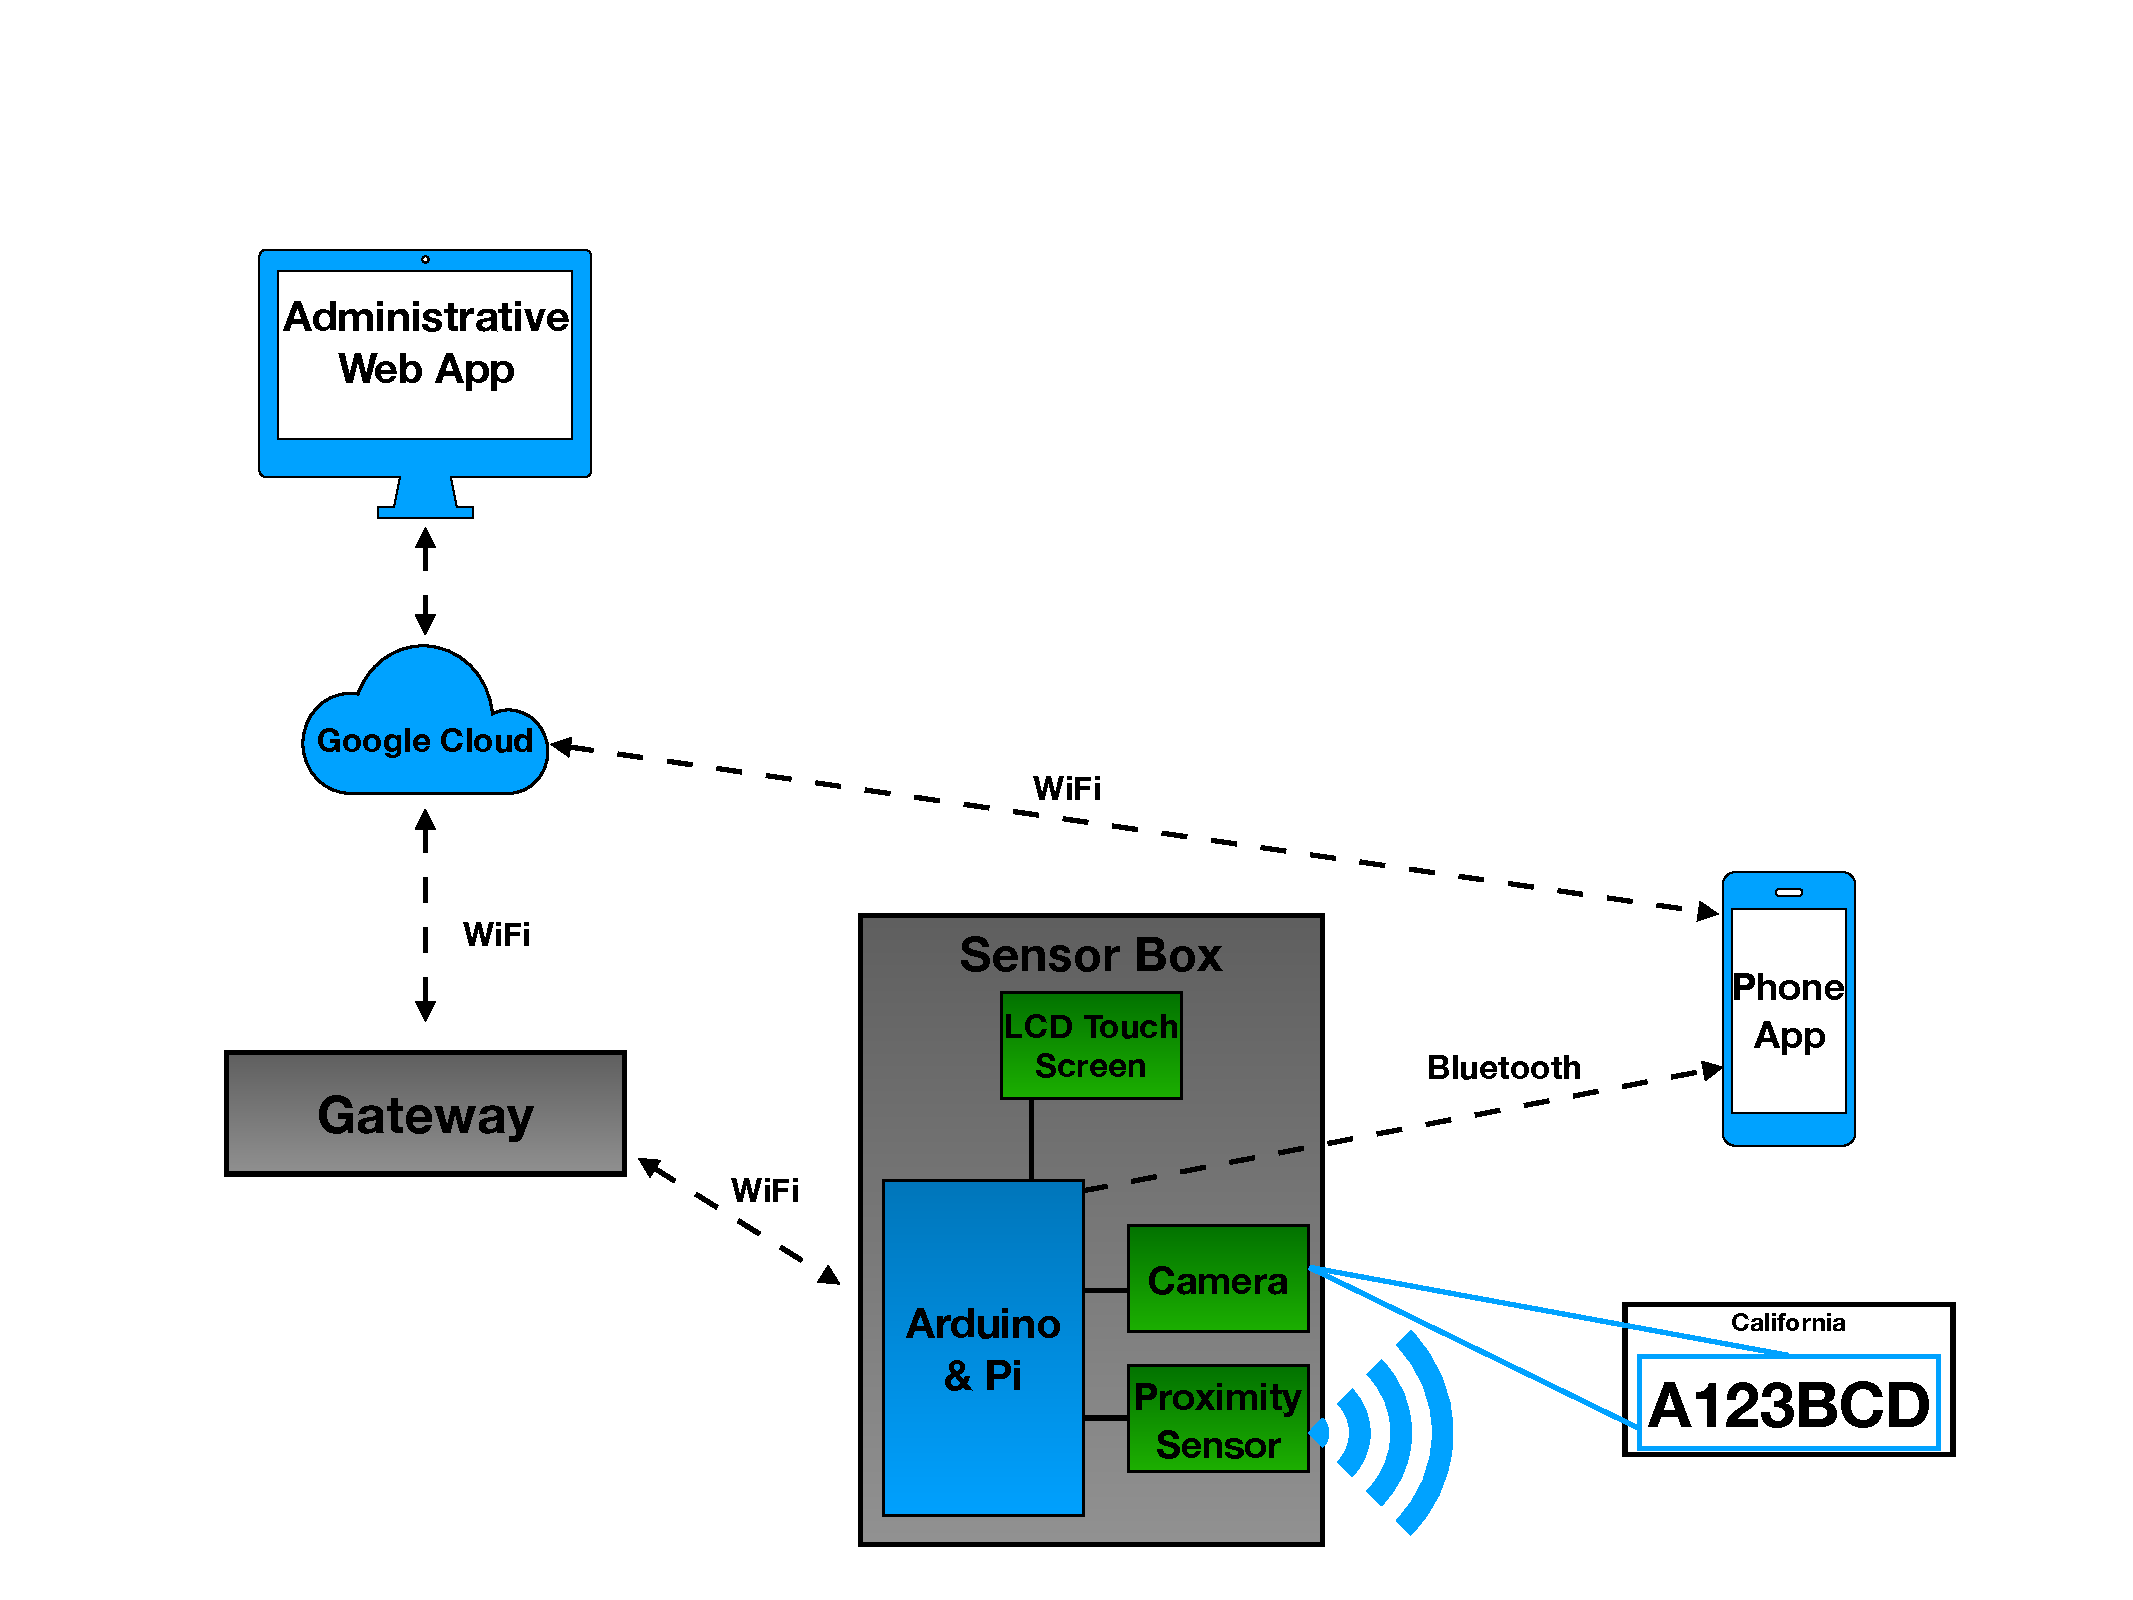
\includegraphics[width=15cm]{NoTitle_BlockDiagram_CE123_tfine.pdf}
\caption{Top Level Block Diagram}
\label{adminReserve}
\end{figure}

In order to describe our project with a high level of abstraction, the project can be broken into several subcategories that form the pieces of the puzzle. Here are the several parts that will make up our design:

\begin{itemize}
  \item Parking Lot Sensor: In order to determine if a spot is vacant or occupied, our group will use a sensor placed at the spot to detect whether an object is currently positioned at that particular spot. In order to scale this project, every spot in a parking lot will have a sensor placed to perform the same operation. 
  \item Camera: A small camera is placed on the parking lot to take an image of the car's license plate in order to send that number to the cloud for further processing.
  \item Microcontroller: The microcontroller will be the basis for processing and sending data to the cloud from the sensor and camera in the parking lot. Once a user pulls over a vacant parking spot, the sensor will send a message to the microcontroller indicating that the spot is taken. This message is send to the cloud from the microcontroller since it has wifi and cellular capabilities. The microcontroller also has bluetooth, and therefore the user can use the bluetooth functionality on their phone to establish a connection with the microcontroller to authenticate themselves and signal that they intend to park at that spot.
  \item Cloud Database: The cloud acts as the major storage center for data and is the central node of access for all of the other elements in this project. The cloud collects data from each piece in the project and also sends back  the appropriate data when requested from these devices.
  \item Mobile Application: The mobile application acts as the user interface for a client who wants to check for parking spots in an area or authenticate themselves when parking in a spot. The bluetooth beacon on the microcontroller at a parking spot will send a unique URL to the phone to confirm which client is parking at a given spot. The phone directly communicates with the cloud in all other instances. If the user is currently enrolled at UCSC, they can simply enter their Student ID to check if they are allowed to park at the spot, and proceed to leave the car once they get a notification on the phone indicating they are good to go. A guest would have the option to pay for parking also using their mobile device.
  \item Website Application: The parking administration would also have a website application to manage parking spots, set up reservations for special events, or perform other tasks remotely, thus making it an easier experience for not just the user but also the administrators of a parking infrastructure.
\end{itemize}

\section{Project Goals and Objectives}
The goal for our team is to design, impliment and deploy a prototype of this device by the end of the quarter.

\section{Sensor Tower Prototype Design}
\begin{center}
\begin{figure}[H]
\centering
\hbox{\hspace{-1.65cm}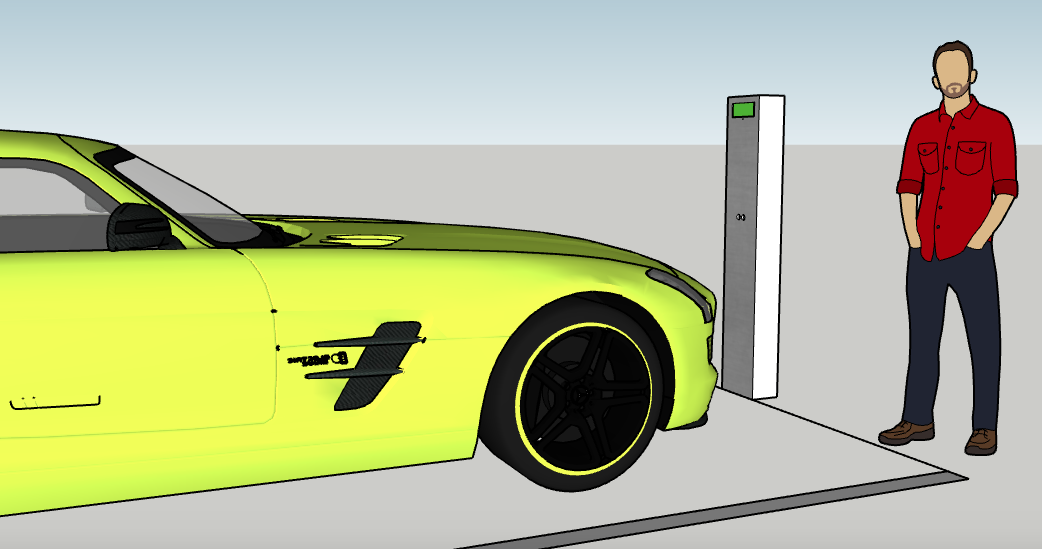
\includegraphics[width=7.5in]{Prototype_Image.png}}
\caption{Parking Space Sensor Tower Prototype Design}
\end{figure}
\end{center}

\section{Design}
The following section will describe in detail the several components that will make up the design for the project and will describe the proposed approach and design for each component in the project.

%--------------------------------------------------------------------------
%start of Scott's stuff

\subsection{Sensor Box} 
The Sensor Box will be placed at each parking spot. It is responsible for sensing when a car has either parked or has left the parking spot. An Arduino equipped with an SR04 distance sensor will be used to identify the status of the parking spot. In addition, the sensor box is a medium for authentication. Authentication can be handle in two ways. First sensor box is equipped with a camera connected to a Raspberry Pi. With the use of computer vision, the Raspberry Pi will be able to identify the car's license plate or tag on the permit (like a QR code). An alternative communication method is via a Bluetooth beacon. This information is then sent to the cloud via a gateway.

To reduce the power consumption, both the Arduino and Raspberry Pi will have a low power mode. Arduino will turn on briefly every 1 to 2 seconds to check the status of the parking spot. If the status has changed, then it will wake up the Raspberry Pi which preform the authentication functions. In addition, since the Administrators needs to have direct access to the Raspberry Pi, the Ardiuno will periodical wake up the Raspberry Pi. The Raspberry Pi will then check the gateway for any service request. This will occur every 30 seconds. 

\begin{figure}[t]
    \centering
    \subfloat[Arduino]{{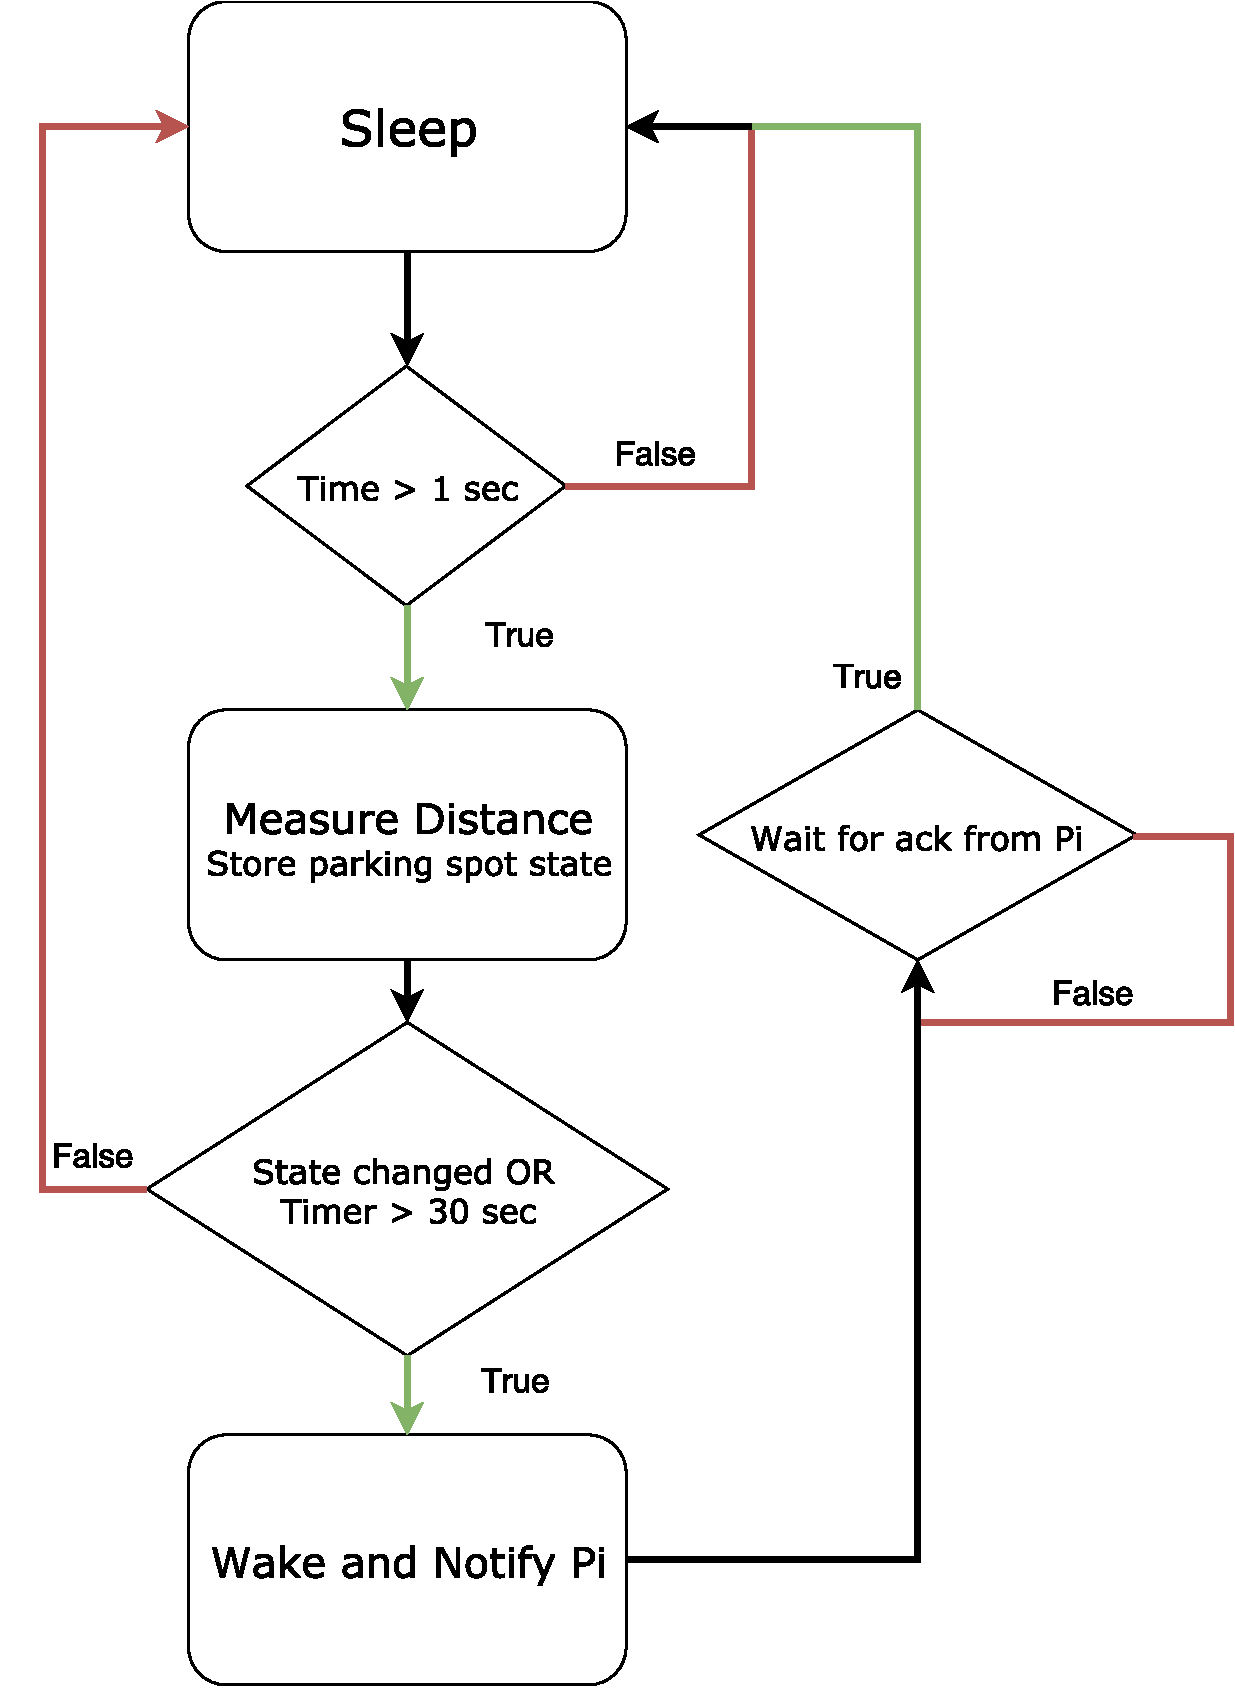
\includegraphics[width=7.5cm]{Arduino_states.pdf} }}%
    \qquad
    \subfloat[Raspberry Pi]{{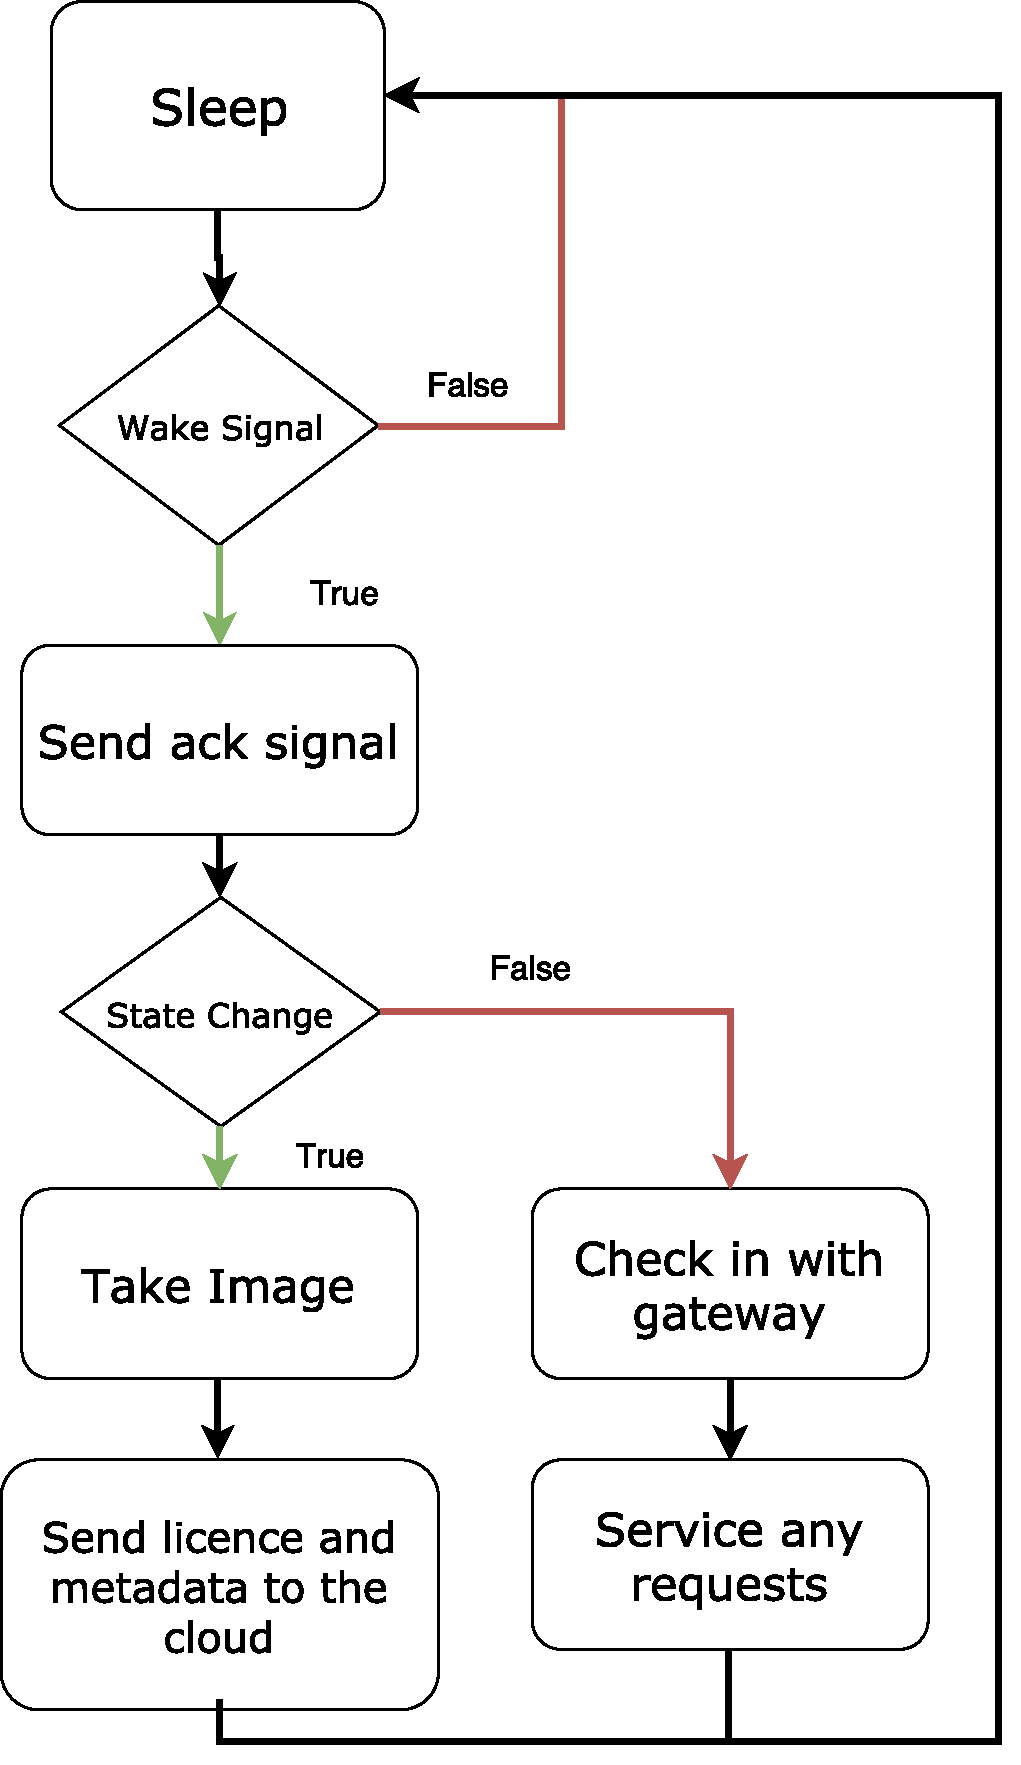
\includegraphics[width=5.5cm]{Pi_states.pdf} }}%
    \caption{State Diagrams}%
    \label{fig:hardware_state}%
\end{figure}

%The Raspberry Pi handles not only handles the local micro-controllers as a central node, but also handles the communication between the hardware and the Cloud. Since the Raspberry Pi doesn't have a sleep mode, the Raspberry Pi would be configured to disable most of its ports and remain at an idle state to maintain the state of minimum power consumption. 

\subsubsection{Connecting the Arduino to the Raspberry Pi}

The Ardiuno is connected to the Rspberry Pi in the following way:

\begin{center}
\begin{figure}[H]
\centering
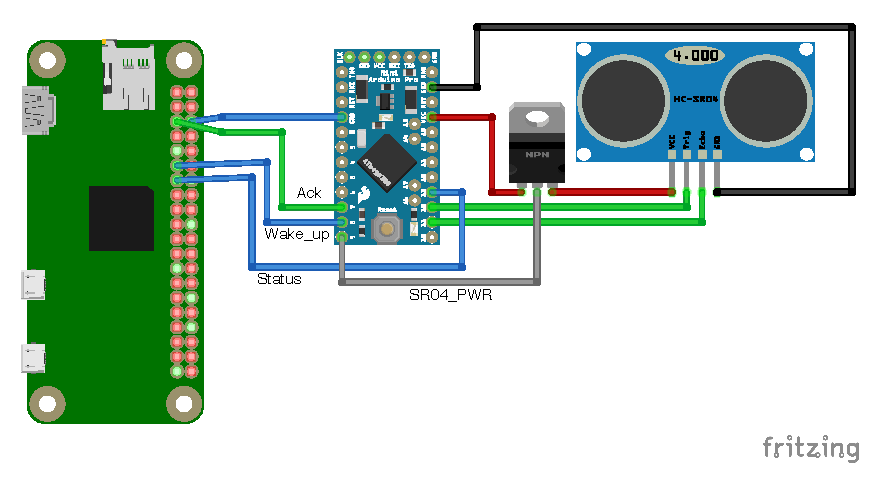
\includegraphics[width=5.1in]{hardware/Wire_Diagram_bb.pdf}
\caption{Sensor Box Wire Diagram}
\end{figure}
\end{center}

\subsubsection{Arduino Sleep APIs}
The following Arduino libraries are needed to implement the sleep state:
\begin{verbatim}
  #include "LowPower.h"
  #include <avr/sleep.h>
  #include <avr/power.h>
\end{verbatim}

Once the libraries have been declared, we can call the following function in void setup() to turn off unnecessary components such analog to digital converters (ADC), SPI and I2C. 

\begin{verbatim}
  power_adc_disable(); // ADC
  power_spi_disable(); // SPI
  power_twi_disable(); // TWI (I2C)   
\end{verbatim}

In the main loop we can use the following function to turn on sleep mode for a specified time. 

\begin{verbatim}
  LowPower.powerDown(SLEEP_1S, ADC_OFF, BOD_OFF); 
\end{verbatim}

In this case the Arduino will turn off for 1 second. Currently the Arduino only uses 50 microamps while in the low power mode. 

\subsubsection{Spot Status API}

The Spot Status API will simply return a Boolean value of the status of the spot. The API will return a TRUE value if the spot is taken, else it will return a false value. Simply call the following function to get the status of the spot:
\begin{verbatim}
  spot_status();
\end{verbatim}

To implement this API we used the following library to interface with the SR04:
\begin{verbatim}
  #include <NewPing.h>
\end{verbatim}
Next the following pre-processor defines are used to define what pins on the Arduino connect to the trig and echo pins of the SR04 sensor and the max distance in cm:

\begin{verbatim}
  #define TRIGGER_PIN  12
  #define ECHO_PIN     11
  #define MAX_DISTANCE 200 //cm
\end{verbatim}

Next, the following command setups up the SR04 which utilizes the defines above: 

\begin{verbatim}
  NewPing sonar(TRIGGER_PIN, ECHO_PIN, MAX_DISTANCE);
\end{verbatim}

The following function will return the distance from the SR04 sensor in centimeters as an integer:
\begin{verbatim}
    sonar.ping_cm()
\end{verbatim}
Lastly, the function is defined to return a true value when the distance is less than 100 cm:
\begin{verbatim}
  return (sonar.ping_cm() < 100 );
\end{verbatim}


\subsubsection{Arduino $\rightarrow$ Raspberry Pi APIs}
Communication between the Arduino and Raspberry Pi will be done via GPIO pins. The Arduino has two output pins. The first pin is a parking status pin. An empty parking space is signified by a low signal and turns high when occupied. The second pin on the Arduino is a wake up pin. This turns high when the state of the parking space changes. The wake up signal will remain high in till it receives an acknowledgement signal from the Raspberry Pi (ack). This is to prevent the Raspberry Pi from missing data sent from the Arduino. See figure 3.2 and 3.3 to see an example of the signals. 

\begin{figure}[h]
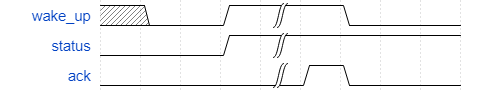
\includegraphics[width=5in]{not_taken_to_taken.png}
\caption{Car pulls into a spot}
\end{figure}

\begin{figure}[h]
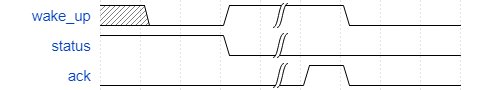
\includegraphics[width=5in]{taken_to_not_taken.png}
\caption{Car pulls out of a spot}
\end{figure}

To output a signal from the Arduino or read a signal from the Raspberry Pi can be done with these functions:
\begin{verbatim}
  digitalWrite(PinName, HIGH); //Write a 1 to PinName
  digitalRead(PinName);        //Read from PinName
\end{verbatim}
The status, wake and ack are connected to the following pins on the Arduino 8, 13 and 7 respectively. 

\subsubsection{Raspberry Pi $\rightarrow$ Arduino}

The Pi will periodically check to see if the Arduino has requested the Raspberry Pi to wake up. First, a setup function is called to set up all the GPIO pin and declare the required variables. This can be done by calling:
\begin{verbatim}
  status_setup();
\end{verbatim}
\noindent
The wake signal can be read with the following function:
\begin{verbatim}
  wake_status();
\end{verbatim}
\noindent
This function returns a true value if the Arduino has requested the Pi to wake up, else it is false. In addition, it clears the wake up signal by sending an ack signal to the Ardiuno.

If the Raspberry Pi has been requested to wake up, then it will then check to see if the status of the parking spot has changed. It can check the status of the spot simply by calling the spot status function:
\begin{verbatim}
  parking_status();
\end{verbatim}

\subsubsection{Raspberry Pi Low Power Mode}

To reduce the Raspberry Pi's idle power consumption, we will disable high power consuming items such as Wi-Fi and USB ports while not in use. The low power mode can be enable and disabled with the following functions:
\begin{verbatim}
  enable_low_power();  //enables  low power mode
  disable_low_power(); //disables low power mode
\end{verbatim}
\noindent
Pleases note that the Raspberry Pi cannot communicate with the cloud nor via USB while in low power mode. The enable low power function also has an exit timer parameter. The parameter has second resolution. Here is an example:     %Therefore, it is imperative that the low power mode 
\begin{verbatim}
  enable_low_power(15);  //enables low power mode for 15 sec
\end{verbatim}

\subsection{Display}

The Display will have similar functionality to the mobile app. They will be able to pay for their spot via a payment processor. Once the mobile app's design has been finalized, this section will be expanded. 

%end of Scott's stuff

\subsection{Gateways}
The gateways serve as a intermediary step between the sensor tower and the cloud, multiplexing data to and from the sensor tower and the cloud. There will be two levels of hierarchy for gateways. Each lower level gateway, (level 2) will be arbitrating data between multiple sensor boxes and the higher level gateway (level 1). The higher level gateway will be arbitrating data between the multiple lower level gateways and the cloud.

The basis for the interconnection between the each of the level 2 gateways and the multitude of sensor boxes is a master slave architecture based off of basic socket protocols, where the slaves are the sensor boxes and the master is the level 2 gateway. 

Similarly for the interconnection between the the level 1 gateway and the multitude of level 2 gateways is a master slave architecture based off of basic socket protocols, where the slaves are the level 2 gateways and the master is the level 1 gateway. 

Both the level 2 and level 3 gateways will however act as both a client and a server depending on the frame of reference. The level 2 gateways will be a server to the sensor boxes, but also a client to the level 1 gateways. Similarly, the level 1 gateways will be a server to the level 2 gateways, but also a client to the cloud server. 

To do this, each of the level 2 gateways must firstly broadcast a signal to determine which sensor towers are in its range. *G (figure out how to determine which towers are assigned to which sensor boxes and how turning the sensor boxes on and off will affect the system and latency to connect and all of that.) Note that this is the only level of hierarchy that must broadcast a signal since all other levels of hierarchy are servers and have static addresses, and are not allowed to turn off.

Once the sensor towers have been identified, the system is ready for use. Using the socket library discussed in the subsequent sections, interconnections over TCP may be established. 

\subsubsection{TCP connection establishment APIs}

\textbf{GatewayServer.py and SensorTowerClient.py:}
The following python module is needed to implement the TCP connection establishment between the client and the server.
\begin{verbatim}
import socket
\end{verbatim}
\textbf{GatewayServer.py:}
After the socket module has been imported we call the function setupServer( ) that establishes the sever socket that will be used, binds the existing socket to its IP address and chosen port number and listens for a given number of connections and returns the socket field descriptor.

\begin{verbatim}
s = socket.socket(socket.AF_INET, socket.SOCK_STREAM)
s.bind((host, port))
s.listen(32)
\end{verbatim}
\textbf{SensorTowerClient.py} 
After the socket module has been imported we call the function setupClient( ) that establishes the client socket that will be used, and initiates connection with via a 3 way handshake, and adds the identified server IP address and port number to the existing socket and returns the socket field descriptor.

\begin{verbatim}
s = socket.socket(socket.AF_INET, socket.SOCK_STREAM)
s.connect((host, port))
\end{verbatim}
\textbf{GatewayServer.py:}
After the setupClient( ) function is called on the client side, the server calls setupConnection( ), which accepts the connection to obtain the parameters of accepted connection, returning the field descriptor for the connection created.
\begin{verbatim}
conn, address = s.accept() 
\end{verbatim}
\textbf{GatewayServer.py and SensorTowerClient.py:}
Once all of the connection establishments and sending and receiving is done, the connection is intimated and completed with function
\begin{verbatim}
conn.close( ) 
\end{verbatim}
on both sides.

\subsubsection{Multithreading APIs}

\textbf{GatewayServer.py:}
The following python module is needed to implement the multithreading APIs to allow for multiple clients to be served concurrently.

\begin{verbatim}
import threads
\end{verbatim}
Once the threads module is imported and after the TCP connection has been established amongst the clients, we can call ClientThread( ), which allows the server to serve all of the clients concurrently, and contains the non blocking send and receive APIs discussed in the next segment. The clients are put into a list, and then threads are created for each of them.

\begin{verbatim}
list_of_clients.append(conn)
start_new_thread(clientThread,(conn,addr))   
\end{verbatim}

\subsubsection{Non Blocking send and receive APIs}

The following python modules are needed to implement the non blocking APIs to allow for the server to receive data from sensor tower and forward to cloud, as well as send the received data from the cloud to the sensor tower. 

\begin{verbatim}
import select
\end{verbatim}

Inside of each of the clientThread( ) function, the select function is called so it is able to arbitrate the different IO concurrently that the server receives including messages from the tower and messages from the cloud. However, at this point I am just using stdin as an input from the cloud.

\begin{verbatim}
#(tentative)
while(True):

	sockets_list = [sys.stdin, s]
	read_sockets,write_socket, error_socket = select.select(sockets_list,[],[])

    	    if read_sockets == s:
           	recvDataSensorTower = s.recv(1024)
		print(“recvDataSensorTower”) #will change to sending Cloud API

     	   else: #  if read_sockets == sys.stdin:
       	   	 recvDataStdin = sys.stdin.readline()
           	 s.send(str.encode(recvDataStdin))
\end{verbatim}
\subsection{Cloud}
\subsubsection{Cloud Summary}
The Cloud will serve as the central node for sending and receiving data to all of the components and establish an important communication link between all of the devices. The Cloud will conceptually have a front-end and back-end section, with the front-end designated for communicating with the user interface of the website and mobile application while the back-end designed to collect and process data coming from the Raspberry Pi(including the image captured from the camera) and the two applications. For this project, we are using the Google Cloud Datastore and the App Engine platforms. Datastore will be used to maintain the databases in figures 3.4, 3.5 and 3.6 which are accessed by The Gateway. A python program will be deployed using App Engine which will be accessed by the user mobile application and and administrator web application.
\begin{figure}[H]
\hbox{\hspace{-1.0cm}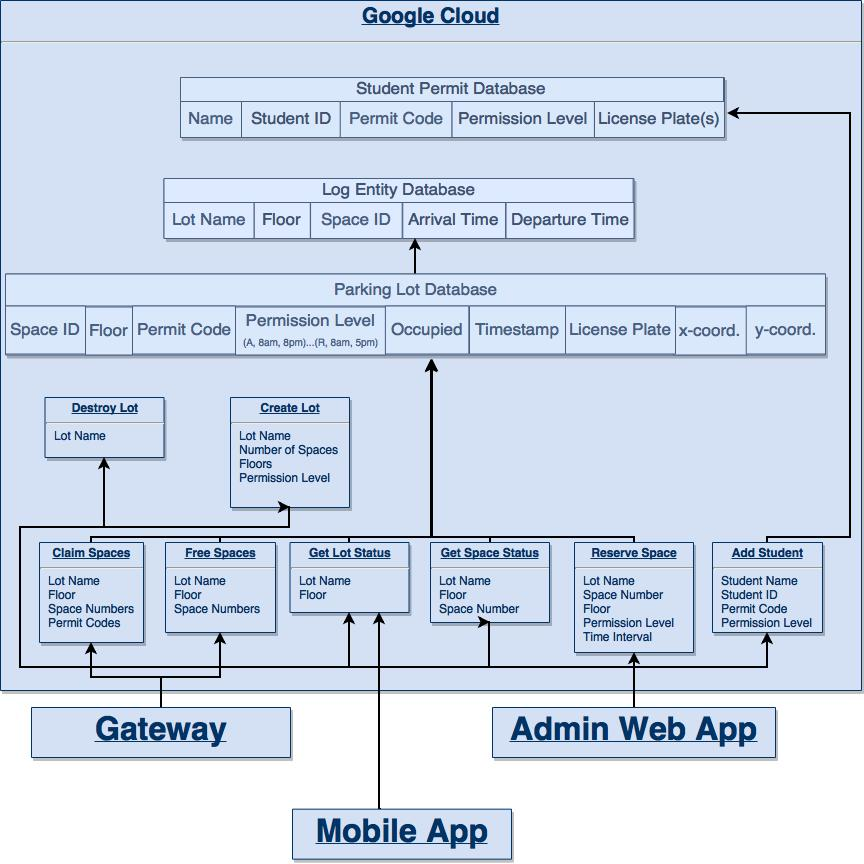
\includegraphics[width=7in]{Cloud_Block_Diagram.jpg}}
\caption{Cloud Data/Flow Block Diagram}
\end{figure}
\begin{figure}[H]
\centering
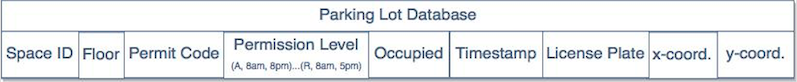
\includegraphics[width=6in]{Structure_DB.png}
\caption{Parking Lot Database}
\end{figure}
\begin{figure}[H]
\centering
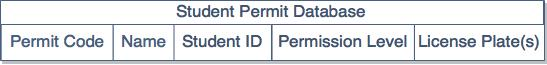
\includegraphics[width=4in]{Cloud_Student.jpg}
\caption{Student Permit Database}
\end{figure}
\begin{figure}[H]
\centering
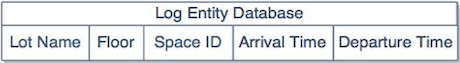
\includegraphics[width=4in]{Log_DB.png}
\caption{Log Entity Database}
\end{figure}

\subsubsection{Gateway to Cloud APIs} 
When a car has pulled into a parking space, the sensor box will send the permit code that has been deciphered via computer vision and its space ID to the Gateway. The gateway will then forward all the claimed spaces along to the Google Cloud Datastore to be added into the structure database. Since this function will be executed by the Gateway, it needs to be able to work with however many spaces the gateway communicates with. Thus, this function will take an array of space numbers and permit codes, so it can update multiple spaces with one function call.
\begin{itemize}
  \item claim\_spaces : space\_num[ ] | code[ ] | occupied | timestamp 
  \end{itemize}
When a car has left a parking space, the sensor box will send its space number to the Gateway, which will then forward all the spaces that have become open to the structure database to be updated.
\begin{itemize}
  \item free\_spaces : space\_num[ ] 
  \end{itemize}
The Administrator has the ability to request a picture from any spot by indicating a parking lot, a floor number if applicable, and a space number. This request will be sent to the Gateway, which will then route the request to the corresponding sensor box and send it back up thru the gateway, to the App Engine and back to the Administrator. 
\begin{itemize}
  \item get\_spot\_pic : space\_num[ ] 
  \end{itemize}
  
\subsubsection{Administrator Web App to Cloud APIs} \label{cloudAdminAPIs}
The Administrator can create a parking lot simply by giving it a name, the number of floors, number of spaces, and the desired permission level of the parking lot.
\begin{itemize}
  \item create\_lot : space\_num[ ] | lot\_name | permission\_level | floors
  \end{itemize}
The Administrator has the ability to select any space to reserve if, for instance, there were a guest speaker coming to a conference. Given a lot name, floor number if applicable, space number, permission level, and span of time that the space will be reserved for. After the time period expires, the space will then return to its default attributes. 
\begin{itemize}
  \item reserve\_space : lot\_name | space\_num[ ] | floor | permission\_level | start\_time | end\_time
  \end{itemize}
Administrator wants to add a student to the database of students along with their corresponding parking permission level
\begin{itemize}
  \item add\_student : name | student\_ID | permission\_level | code
  \end{itemize}
Administrator wants to view the status of a lot
\begin{itemize}
  \item view\_lot\_status : lot\_name | floor
  \end{itemize}
The Administrator can also erase any lot from the database by specifying the lot name. 
\begin{itemize}
  \item destroy\_lot : lot\_name
  \end{itemize}
The Administrator has the ability to request a picture from any spot by indicating a parking lot, a floor number if applicable, and a space number. This request will be sent to the Gateway, which will then route the request to the corresponding sensor box and send it back up through the gateway, to the App Engine and back to the Administrator. 
\begin{itemize}
  \item get\_spot\_pic : lot\_name | space\_num | floor
  \end{itemize}
At any time the Administrator can see the status of any space in any lot. This information would include the Parking Lot name, floor, space number, permission level, the permit code of the student, and the license plate number currently in the space.
\begin{itemize}
  \item get\_space\_attributes : lot\_name | space\_num | floor
  \end{itemize}
This function will be executed if the administrator wishes to see any changing trends in parking over a specified timeframe. The administrator will be able to view parking statistics at the hour scale over the quarter or academic year. 
\begin{itemize}
  \item get\_parking\_stats : lot\_name | start\_date | end\_date
  \end{itemize}

\subsubsection{Mobile App to Cloud APIs} \label{cloudMobileAPIs}
The Client using the mobile application has limited access from the cloud to perform tasks like view the status of a parking lot and can send information to check against what is registered in the cloud. Here are the API's that will be used for this interface:
\\\\
User is a guest that wants to register themselves on the cloud:
\begin{itemize}
  \item add\_guest : name | code
  \end{itemize}
\\\\
User is a student that wants to log in:
\begin{itemize}
  \item student\_login : student\_ID | password
  \end{itemize}
\\\\
User wants to view the status of a lot:
\begin{itemize}
  \item view\_lot\_status : lot\_name | floor
  \end{itemize}
\\\\

%---------------------------------------------------------------------------------

\subsection{Computer Vision}
Integrated into the Raspberry Pi, the Computer Vision part of this project aims to convert the input image from a connected camera into a character string which is the license plate of the vehicle. This part incorporates with the current OpenCV library and simple CNN's aiming to have a higher accuracy on recognizing the license plate correctly.

\subsubsection{System Design}
The Computer Vision part would be a part of the program written in python so that when the function get\_license\_plate is called, the raspberry pi wait half a second for the camera to warm up. Then using the camera to take a photo of the car including the license plate and then save the image as a jpeg file for the image processing  module to process this image. After processing the image,this function would return a string representing the license plate of the car and then transmit the data with its accuracy to the gateway or the cloud
\subsubsection{Flow Chart}

\begin{figure}[H]
\centering
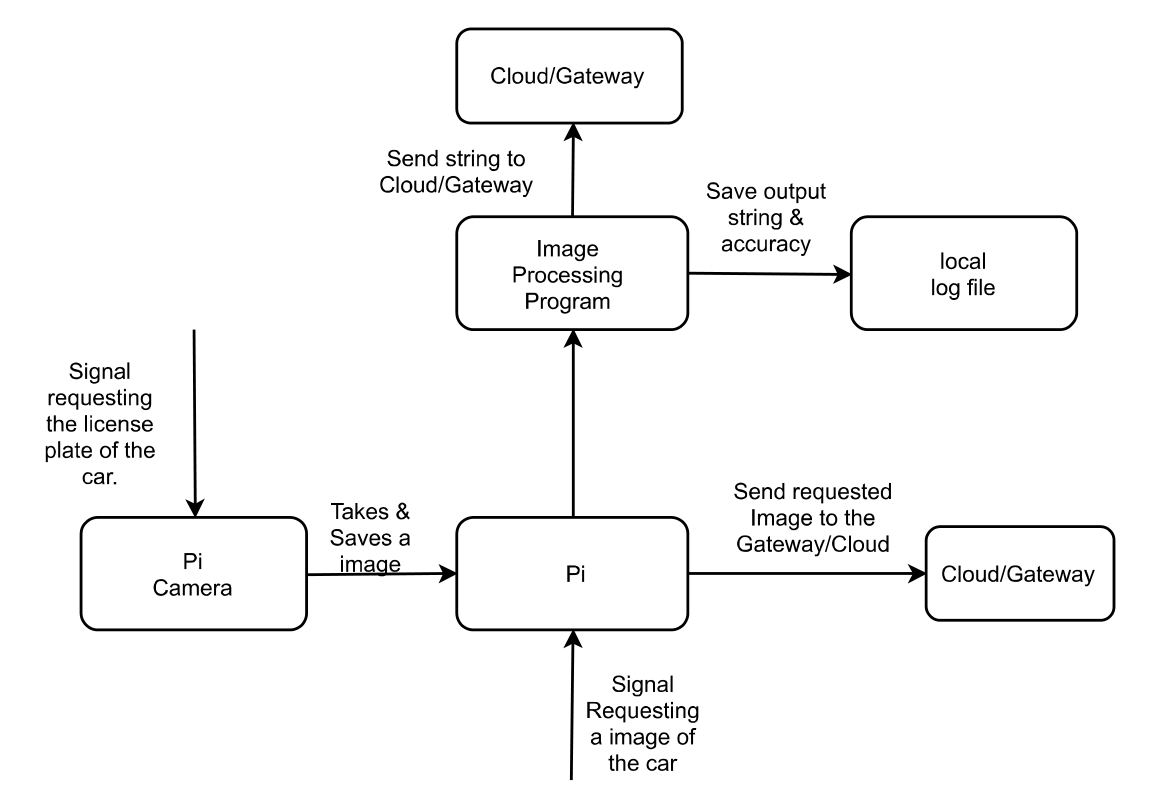
\includegraphics[width=6in]{CV.png}
\caption{Computer Vision Flowchart}
\end{figure}

\subsubsection{Dependent libraries}
Tensorflow: an open-source software that would be used for machine learning application to train a neural network to do the image processing and recognize the license plate of the parked car.
Python: The majority of the Computer Vision part would be written in the Python programming language.

\subsubsection{APIs}
\verb+get_license_plate()+\newline
This function takes a picture and do the image processing on the picture then return a string represent the license plate / code, and a double representing the accuracy.\newline
\newline
\verb+request_image(period)+\newline
This function takes in the period of day and resend all the pictures taken at that hour to the gateway or the cloud for the administrator \newline
\subsubsection{Details of the API}
In the Computer Vision part of the design, A function call get\_license\_plate() would be called to get the license plate of the car. To return both a string that represent the license plate and the accuracy generated by the CNN neural network, a sturct as a pair is needed that pair.first is the string and pair.second is the accuracy
\newline
Other than getting the license plate, the Computer Vision part also support taking an jpeg image as big as 1-2MB that would allow the administrator to see what's going on in the parking lot. The Computer Vision part also supports giving a live stream at the parking spot which would allow the administrator to see to video as high as 15 frames per second. The live stream of the parking spot would be greatly constrained by the data transfer rate so this idea would be left for the future development depending on the bandwidth of the communication.


%---------------------------------------------------------------------
\subsection{Mobile Application}
The mobile application is the one that will be used by the client who wants to park at a spot. The application will give the user information about how many parking spots are open at a particular parking lot, look up what information about them is stored in the cloud database, authenticate themselves with the bluetooth beacon on the gateway,and have a payment option if the client is a non UCSC student or staff member.

\subsubsection{App Design}
The mobile application for this project allows the user to access limited amount of information from the cloud to make decisions as to where to park and updates them with real time data to see whether a spot's status has changed from occupied to vacant or vice versa. As a result, the user will have the power to access a lot of information but not really send much data at all. The following pictures will show the design for each screen in the app and describe what functionalities they have.
\\\\
\textbf{Screens 1 and 2: Welcome Page and Student Login}
\begin{figure}[H]
    \centering
    \subfloat[Welcome Page]{{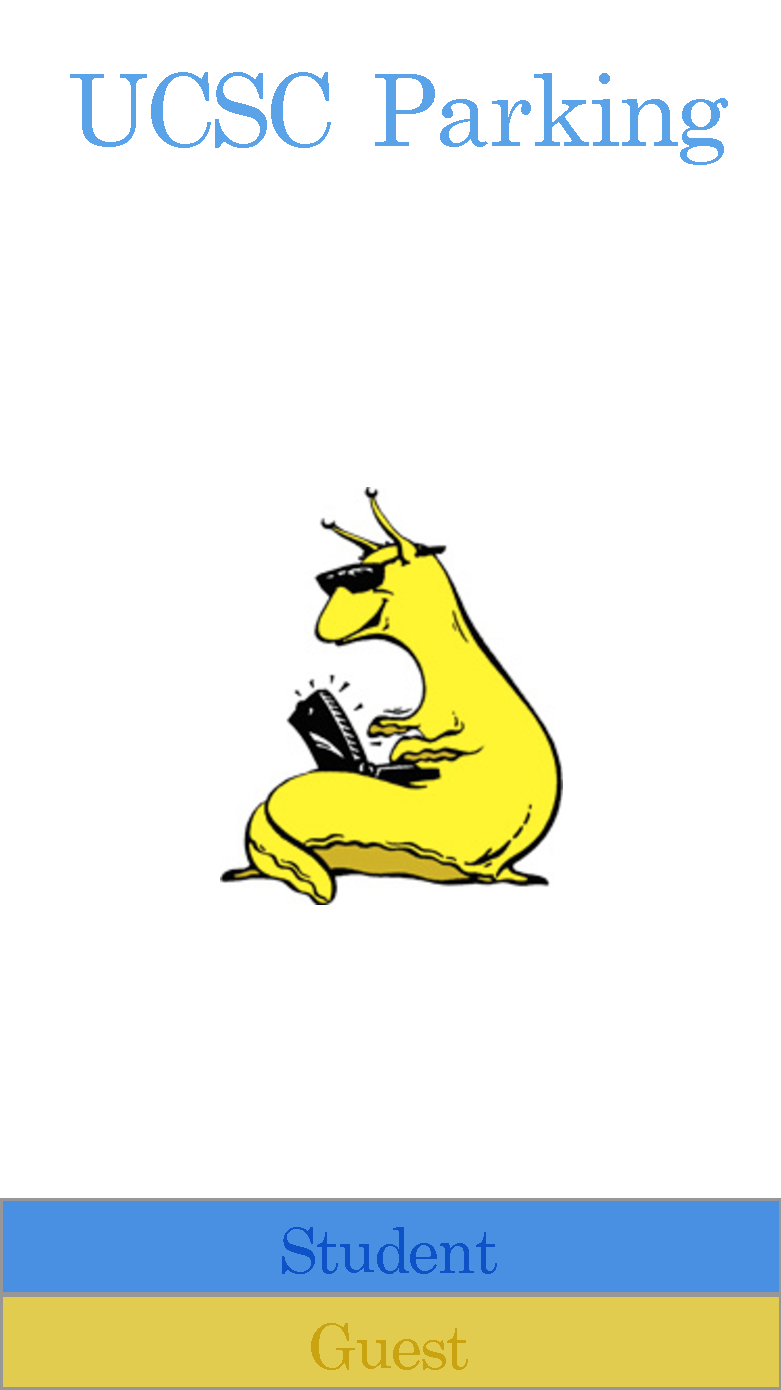
\includegraphics[width=4cm]{MobileAppPics/App Design 1.pdf}}}
    \qquad
    \subfloat[Student Login Screen ]{{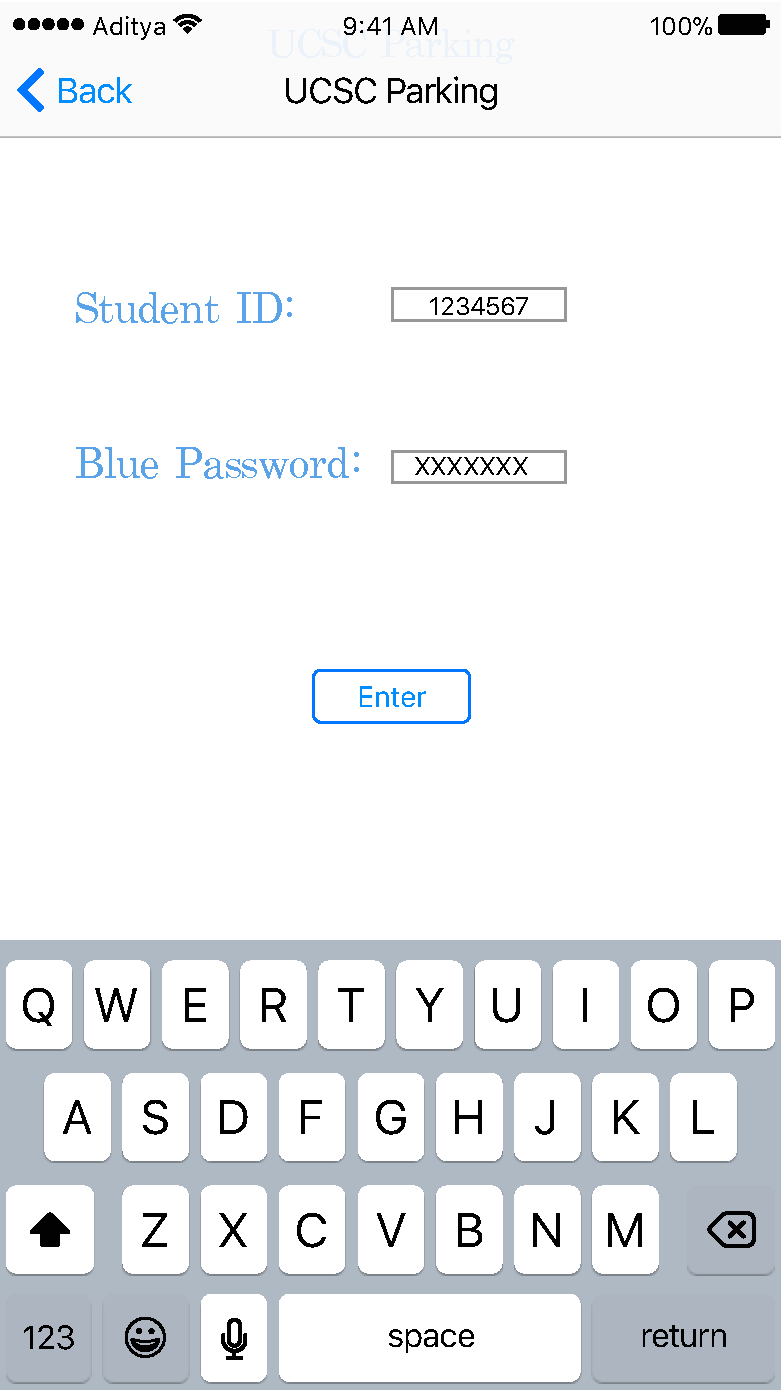
\includegraphics[width=4cm]{MobileAppPics/App Design 2.pdf}}}
    \caption{Screens 1 and 2}
\end{figure}
\\\\
The Welcome Page will be the first screen that the user will see when they open the app. It displays a simple opening splash screen and asks the user to state whether they are a currently enrolled student at UCSC or if they are a guest trying to find parking on campus.
\\\\
The Student login page will open only if the user presses the Student button on the welcome page. Here, the student will enter their Student ID and their Cruz blue ID password in order to authenticate themselves. This information will be sent to the cloud in order for processing.
\\\\
\textbf{Screens 3 and 4: Grouped Parking Lots Page and focusing on a specific lot}
\begin{figure}[H]
    \centering
    \subfloat[Parking Lots]{{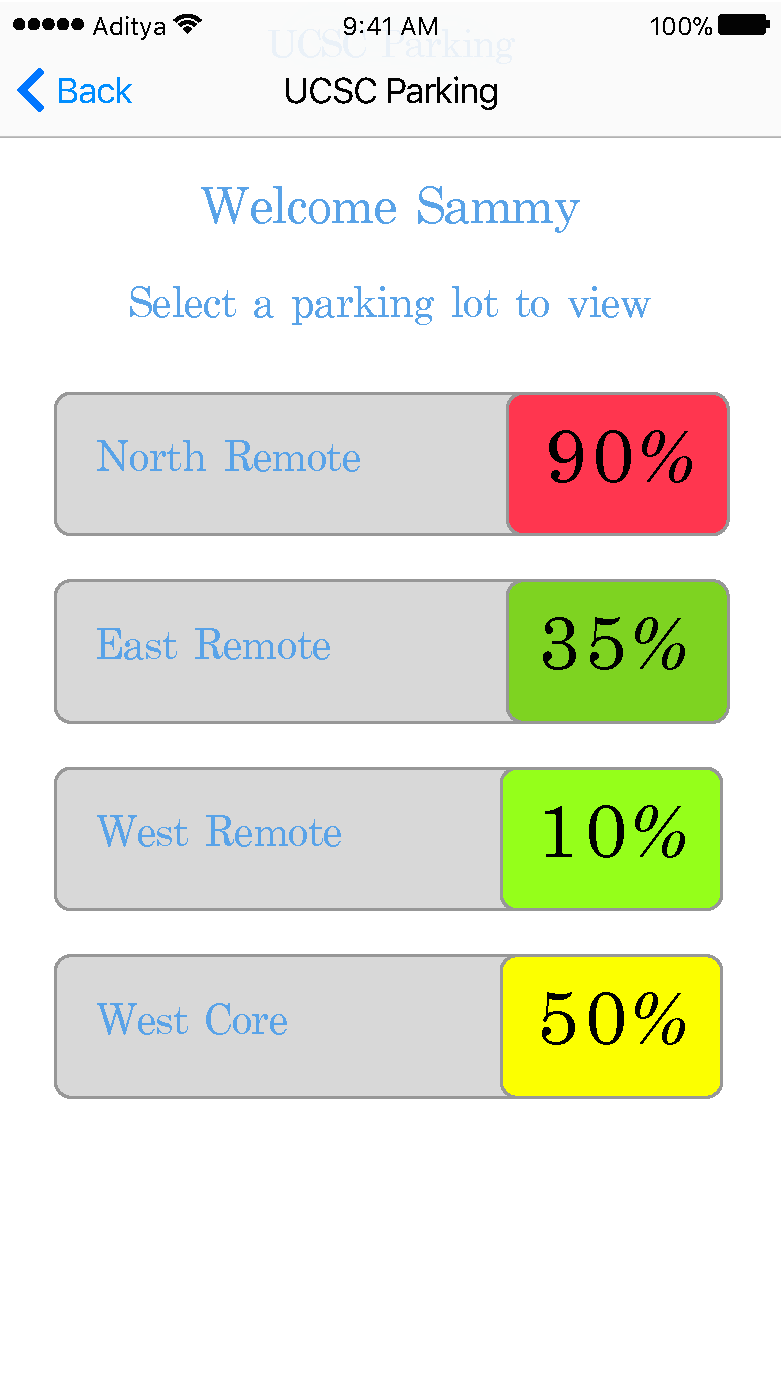
\includegraphics[width=4cm]{MobileAppPics/App Design 3.pdf} }}
    \qquad
    \subfloat[West Remote]{{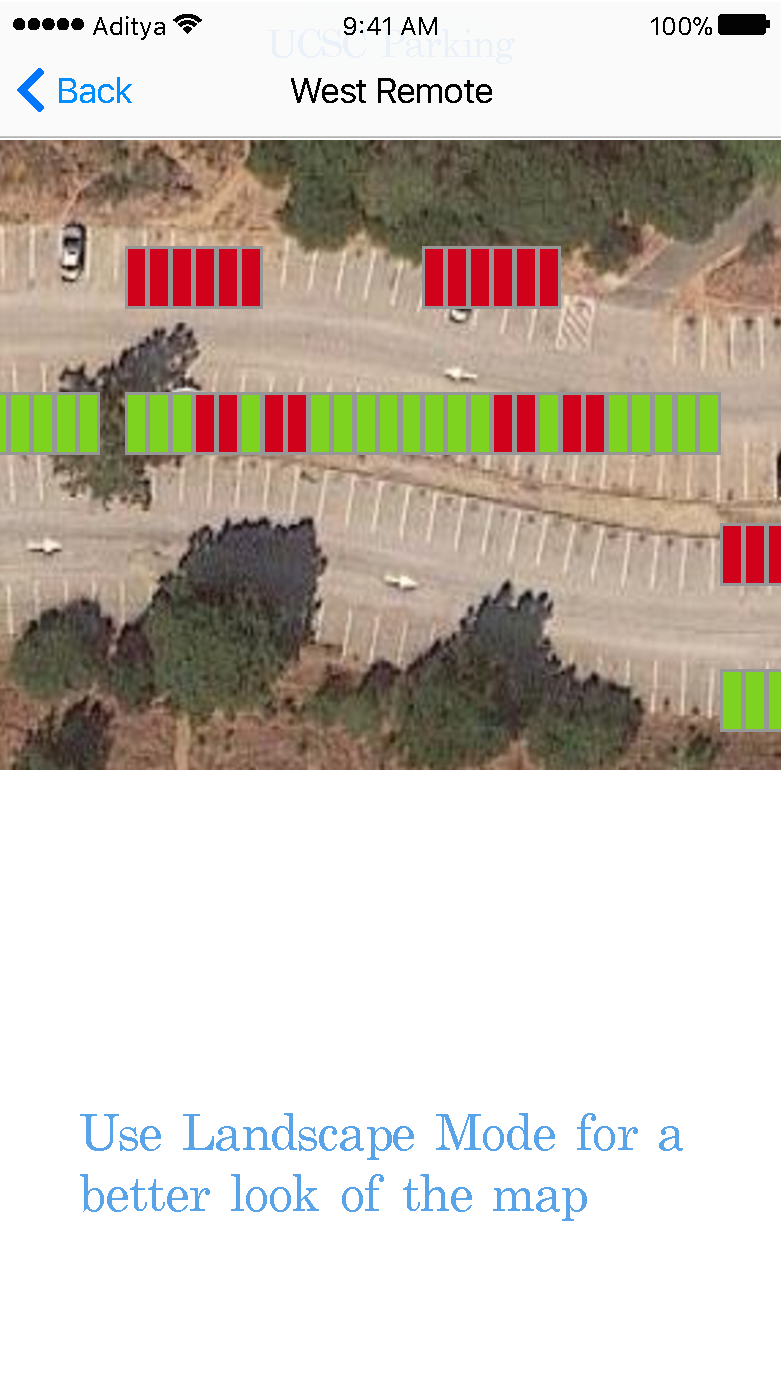
\includegraphics[width=4cm]{MobileAppPics/App Design 7.pdf} }}
    \caption{Screens 3 and 4}
\end{figure}
\\\\
The Grouped Parking lots page will showcase the 4 major parking lots on campus (North,West,East Remote and Core West) and display to the user the percentage of parking spots that are filled up during that given time. The colors correspond to how full a parking lot is, red indicating a high percentage and green indicating a low percentage. Using that spectrum of colors, it ranges from a dark green for 0\%, yellow for 50\% all the way to dark red for 100\%
\\\\
The right figure shows an example of what the screen would look like if the user were to click the West remote button in the previous screen. A map of west remote would open up and each spot will be represented with a green or red rectangle to indicate if the spot is vacant or occupied. In our app design, a red would indicate the spot is taken and a green would indicate that it is currently vacant. The top screenshot is displayed in potrait mode, but if the user wants a better view of the parking lots, switching over to landscape will serve as a better option. Here is how it will look in landscape mode:
\begin{figure}[H]
\centering
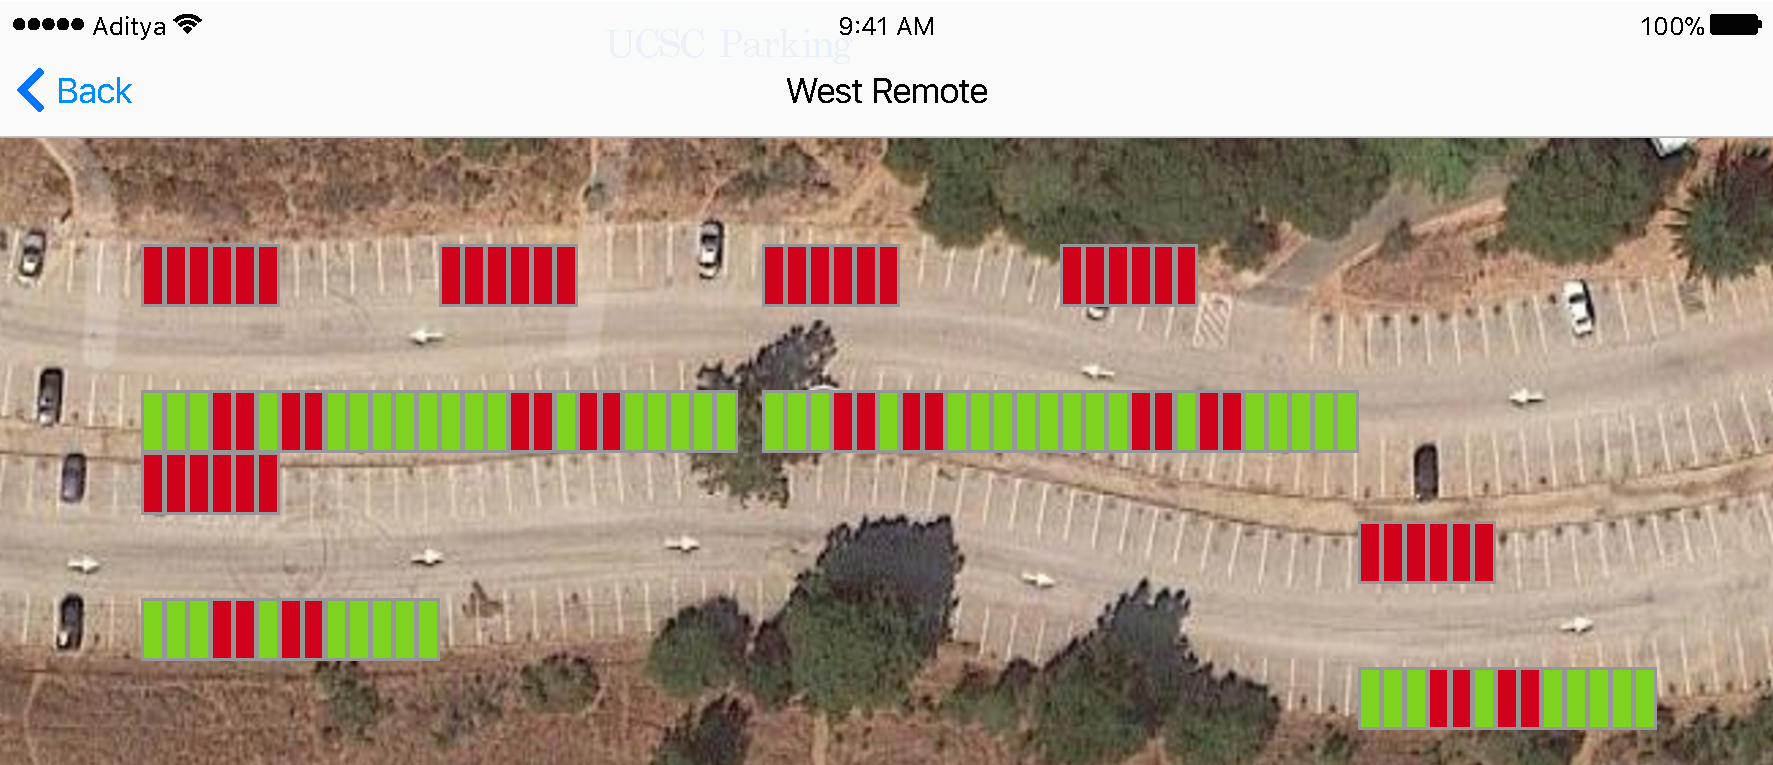
\includegraphics[width=15cm, height=5.5cm]{MobileAppPics/App Design 4.pdf}
\caption{Viewing the West Remote Parking lot in landscape mode}
\label{adminReserve}
\end{figure}
\\\\
\textbf{Screens 5 and 6: Payment Screen and Authentication Screen}
\begin{figure}[H]
    \centering
    \subfloat[Payment Page]{{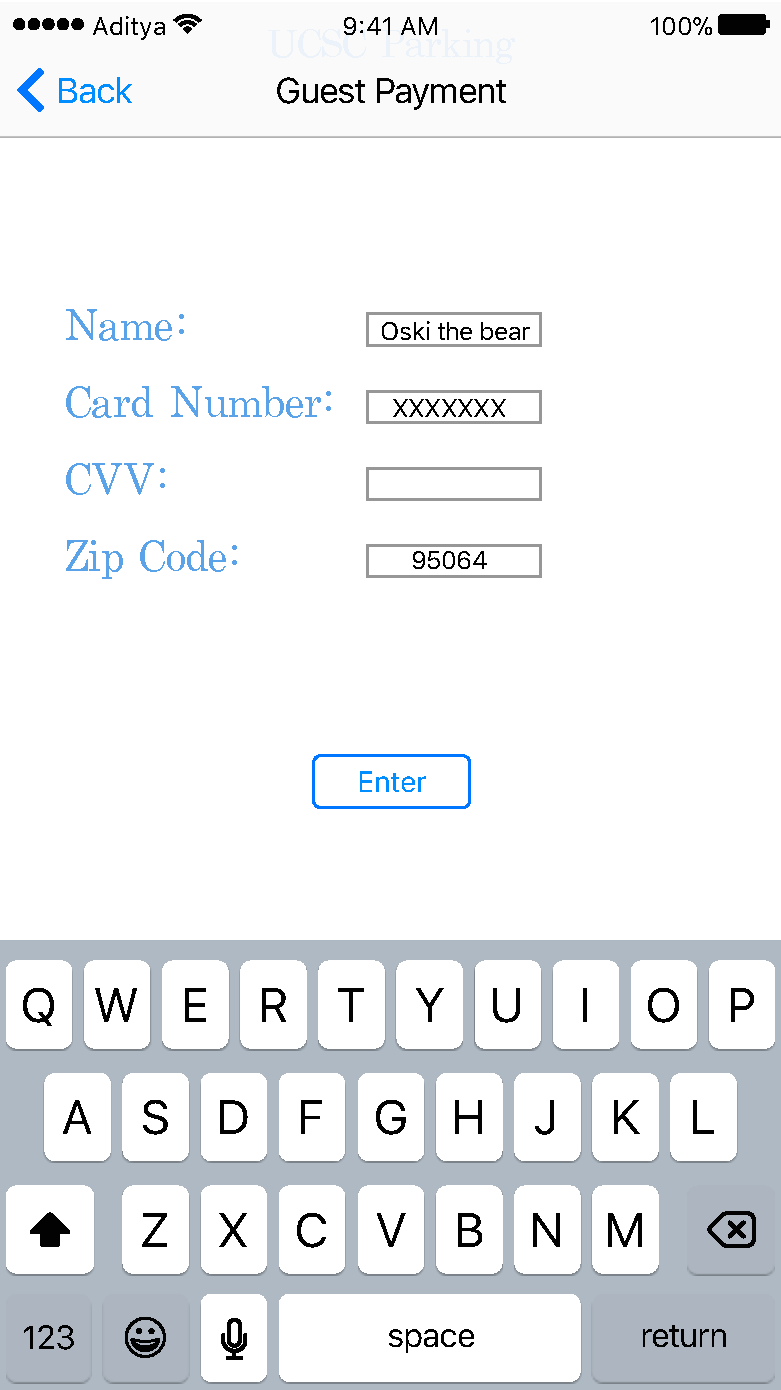
\includegraphics[width=4cm]{MobileAppPics/App Design 5.pdf} }}
    \qquad
    \subfloat[Authentication ]{{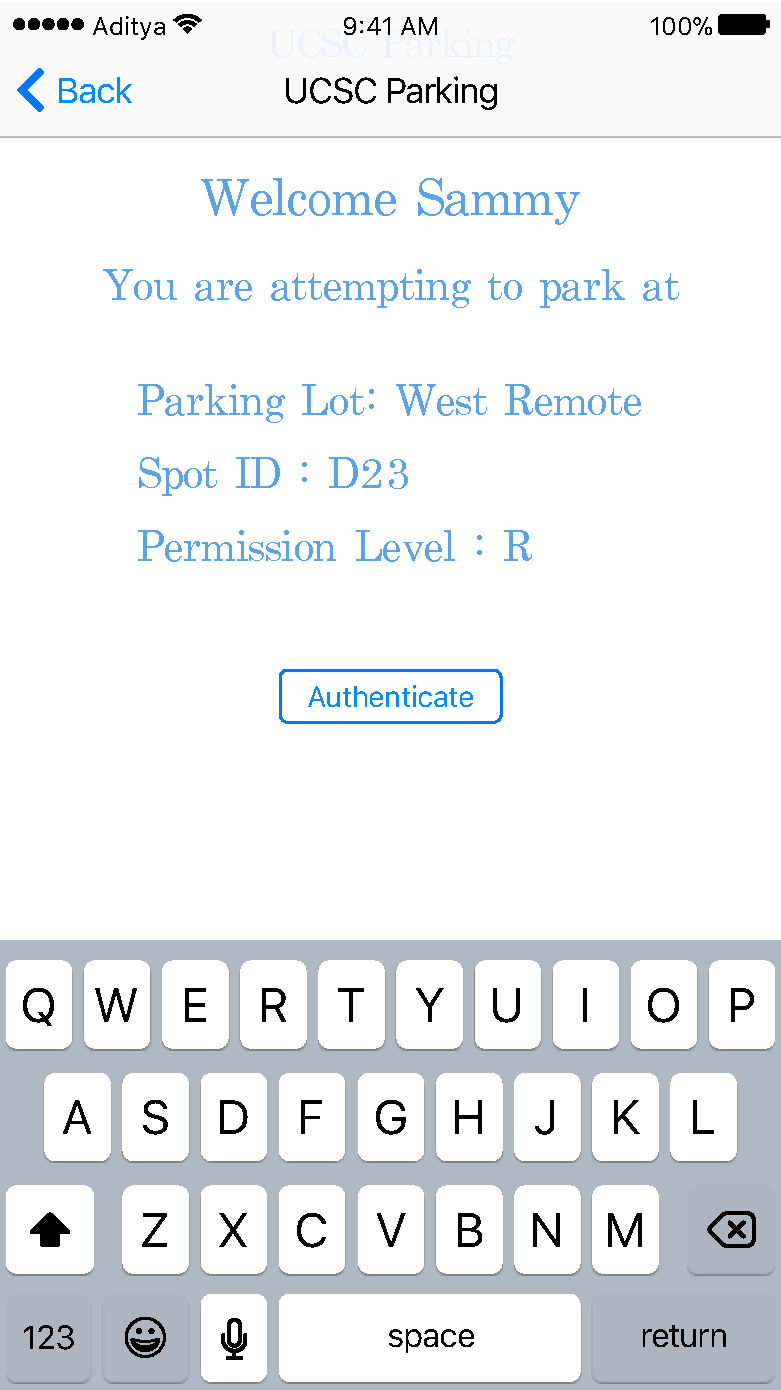
\includegraphics[width=4cm]{MobileAppPics/App Design 6.pdf} }}
    \caption{Screens 5 and 6}
\end{figure}

Both the screen displayed will only pop up when a user has parked their car in a spot and established a connection with the beacon. When the bluetooth beacon sends a unique URL to authenticate with the user, one of the two screens from above will be displayed.
\\\\
If the user is a guest, the payment screen will be prompted asking them to enter their payment information to process how much they will have to pay for parking.
\\\\
If the user is a student, the authentication screen will pop up instead showing all of the information about them that is stored in the cloud to confirm their credentials and parking status. The user can review this information and confirm that they want to park at this spot by pressing the authenticate button. This is how the app design will look for our project.

\subsubsection{App Flowchart}
For our mobile application to function properly, we have designed it to follow a certain protocol as defined in the protocol to navigate through the several screens appropriately and function seamlessly. Here is our flowchart for the app:

\begin{figure}[H]
\centering
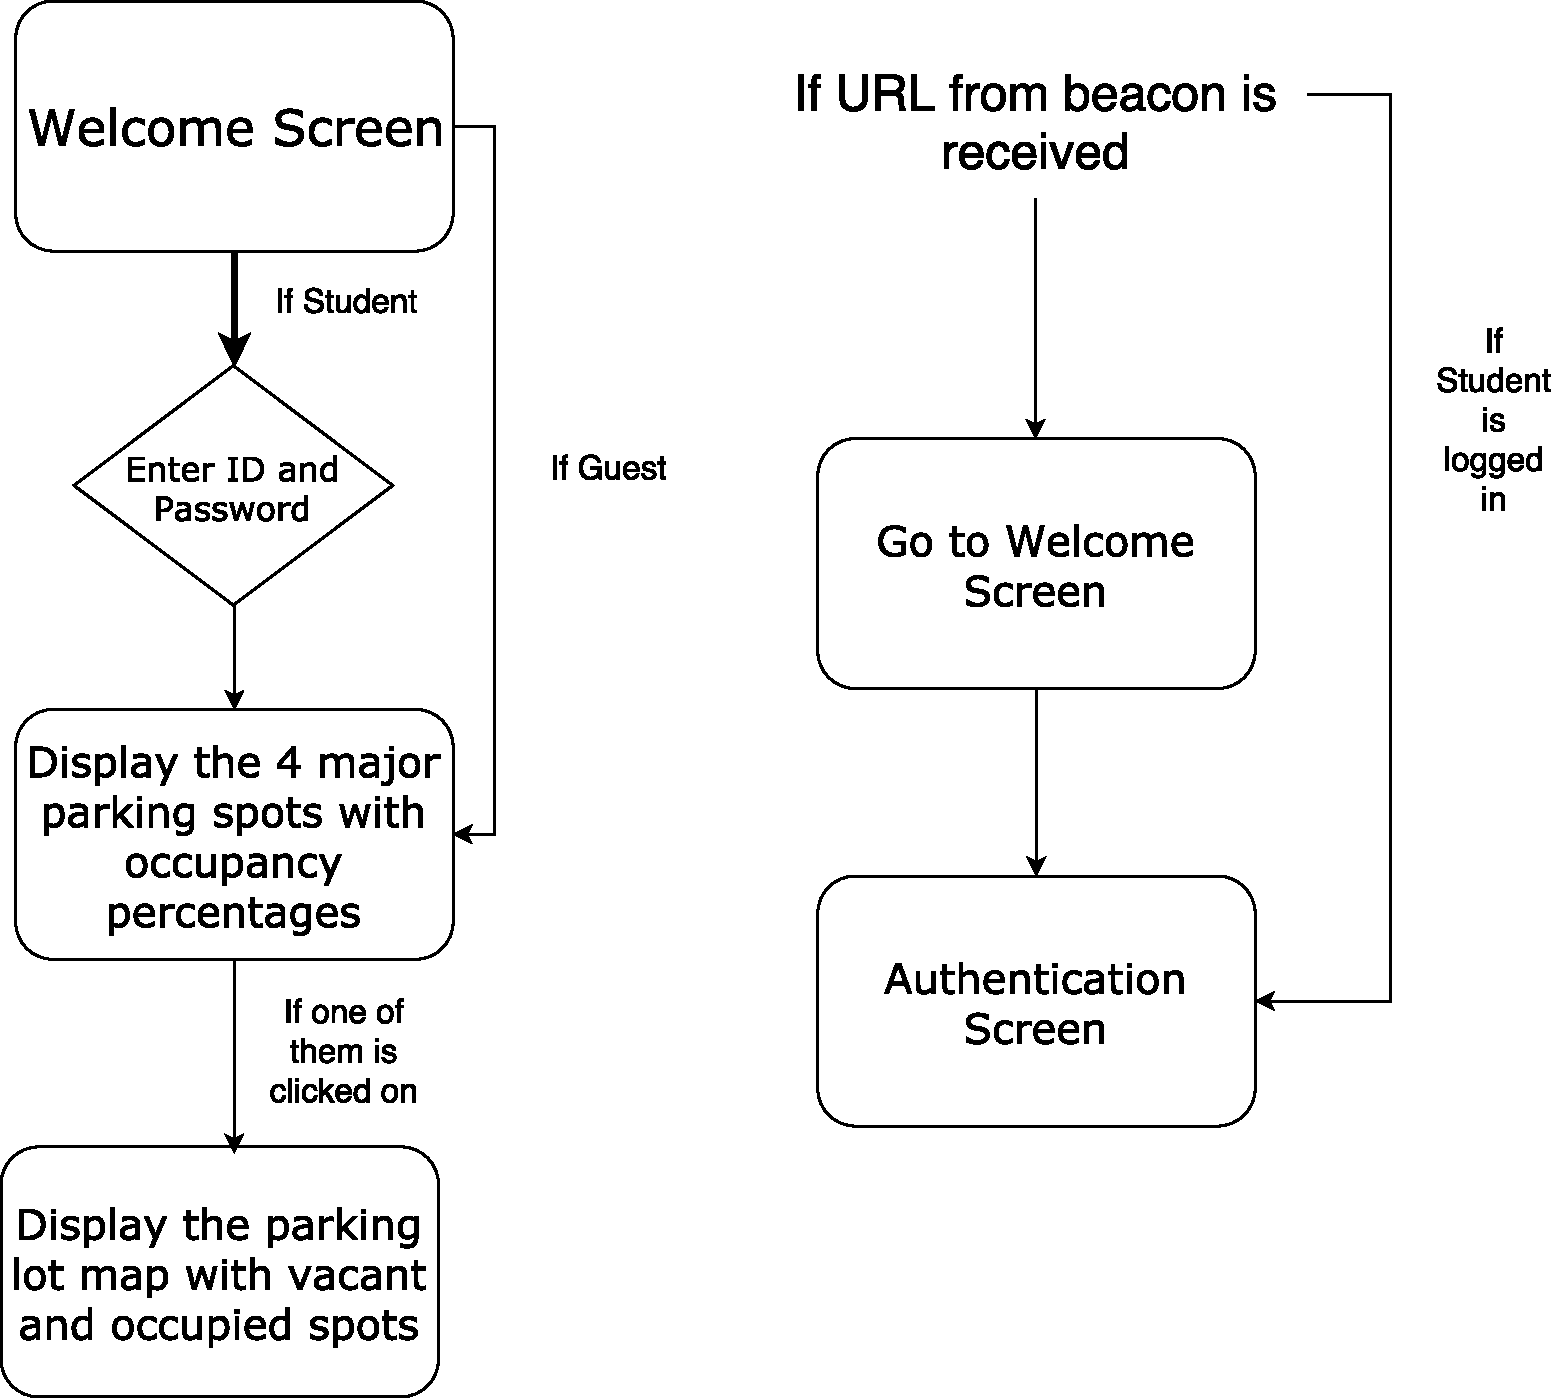
\includegraphics[width=5in]{MobileAppPics/Mobile App Flowchart (3).pdf}
\caption{Mobile App Flowchart}
\end{figure}

As described in the design section, the app will start off with a welcome screen and will prompt the user to state if they are a student of guest. If they are a student, the student login page will pop up before going to the parking lots page. If they state to be a guest, the app will directly go to this page. Finally, the user can view the parking lot of their choice in more detail if they choose to.
\\\\
If the student is already logged in, the app will jump straight to the authentication page at any time if it obtains the URL from the bluetooth beacon since this will be optimal for the user since they have already parked at a spot of their choice and simply want to authenticate themselves before exiting their vehicle. If they are not logged in or are using the app as a guest, the welcome page would pop up again and then ask whether they are a student or guest before going to the authentication screen.

\subsubsection{App Software}
In order to write this program and deploy its first iteration, our plan is to use Android studio and design an Android only app initially. To design the app's graphic user interface (GUI), we plan on writing a css file that is provided in Android studio and to design the app functionality, we plan on writing it as a java file in the same program. Android Studio provides several library API's that makes it easy to connect it with Google Cloud since Android is part of Google. Once the Android version of the app is written and tested, the plan is to also write an iOs version of the app to expand the platforms on which this app can run on.
\\\\
The screenshots of the app seen above were designed using an application called "sketch", which allows the user to draw detailed designs of how their app will look like before implementing it on a program. Sketch only allows the user to design apps for an iOs device, and therefore the screenshots indicate how the app would look like for an iPhone version of the app. However, similar architecture will be used to design the app for Android as well.

\subsubsection{Sending and receiving data}
The Mobile app will be heavily sending and receiving data from our cloud. During this process of interchanging data, well formatted and structured data is required. We plan to use JSON parsing for carrying out this process since it is good and well structured, lightweight and easy to parse and human readable.
\\\\
The mobile application is responsible to send information to the cloud if the user is a student and enters their credentials. Our JSON object would be formatted in this following way:
\\\\
\textbf{"studentinfo": [
\\
"id": "1234567",
\\
"spasswd": "bananaslug123"
\\\\
}
The cloud will process this information and send back the name of the client to confirm who is using the app. Once again, we will use a JSON object to send back this information to the phone. Similarly, the mobile app will receive a JSON object from the cloud after the bluetooth beacon sends the URL to the phone to authenticate the user. This JSON object will contain information of the parking lot and the client's parking privileges to authenticate if they can park in that spot. This JSON object will look as follows:
\\\\
\textbf{"clientinfo": [
\\
"cname": "Sammy the Slug",
\\
"clot": "West Remote",
\\
"cspotid": "D23",
\\
"cpermission": "R"
\\\\}
One thing to note here is we need to send some of the JSON objects with a level of encryption or security since it will contain sensitive data like the person's password or credit card information. By using a commonly used hash function like \textbf{MD5}, we can resolve this issue.

\subsubsection{Dependent Libraries}
\textbf{crypto-js}: This library in javascript contains a large collection of standard and secure cryptographic algorithms implemented in JavaScript. They are fast, and they have a consistent and simple interface. This will be necessary to process JSON objects that contain a student's blue password or a guest's payment information.

\subsubsection{API's}
The APIs of the mobile application are not so much APIs, but rather calls to APIs that are on the cloud. The cloud server will host written functions and scripts, and the mobile application will simply call the appropriate API based on what information the user desires to see. For the mobile application, our goal is to design the first prototype of the app using Android studio as it enables us to utilize several predefined APIs.These API's will work well with the Google cloud platform since Android is part of Google. For instance, to authenticate a user to the cloud, we will utilize the API called "Interface authenticator". To see more of the APIs that the mobile application can call refer to section 6.4.3 and 6.4.4
%---------------------------------------------------------------------
\subsection{Administrative Application}
The web application is an application that can be run on a browser. The application gives TAPS personnel unlimited access to the information on the cloud. This means they are able to designate parking spots as taken, even if they are not, essentially reserving them for people/events. The application is written in HTML and a series of other languages that are related to HTML including, but not limited to CSS, javascript,and python. In the following pages we have images that help outline the capabilities and the design of the administrative application. We will first begin with logging in to the administrator application.

\begin{figure}[H]
\centering
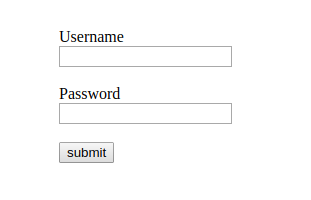
\includegraphics{adminAppPics/loginPage.png}
\caption{The administrator must log in to access the application}
\label{adminMenu}
\end{figure}

For fairly obvious security reasons, the administrator will have to log in. They will be able to set their username and their password, but they will have to type them in every time they want to use the application. This prevents unauthorized users such as students from access the application and abusing it for their own purposes. Once the adminstrator has input their credentials they are then redirected to the main menu of the application.


\begin{figure}[H]
\centering
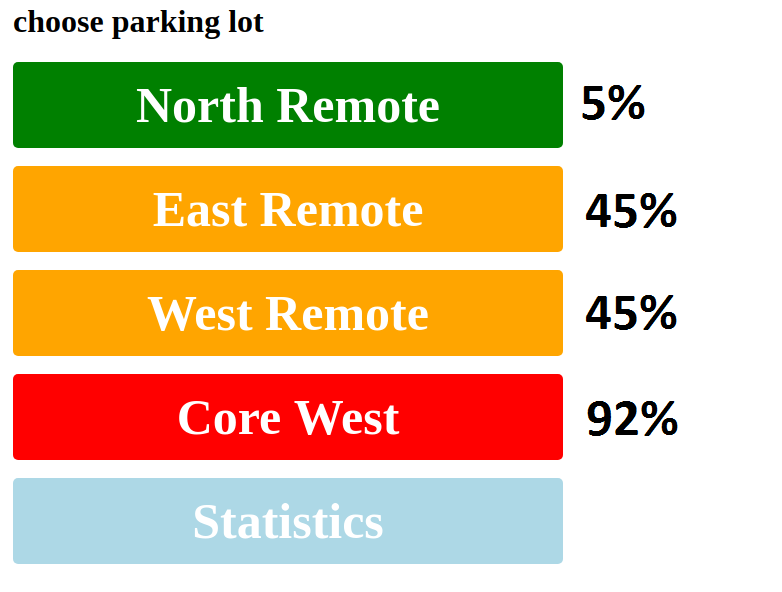
\includegraphics[width=8cm]{adminAppPics/adminMainMenu.png}
\caption{Main Menu}
\label{adminMenu}
\end{figure}

What we see in figure \ref{adminMenu} is a picture of our main menu for the administrative application. We are currently planning on supporting the North Remote, East Remote, West Remote, and Core West parking lots for out project. The color of the buttons reflect the fullness of the parking lot. Green is more empty and red is more full. So as we can see above, the North Remote parking lot is fairly empty. The East and West remote lots are beginning to fill up. And finally, the Core West parking lot is completely full. Then the administrator can click on the lot that they wish to examine. This will redirect them to another page that will contain a google satellite image of the parking lot with little objects overlayed over each parking spot. Then when the administrator clicks on a spot, a little window will show up that will show the details of each spot. Figure \ref{adminLotScreen} shows what this page looks like.

\begin{figure}[]
\centering
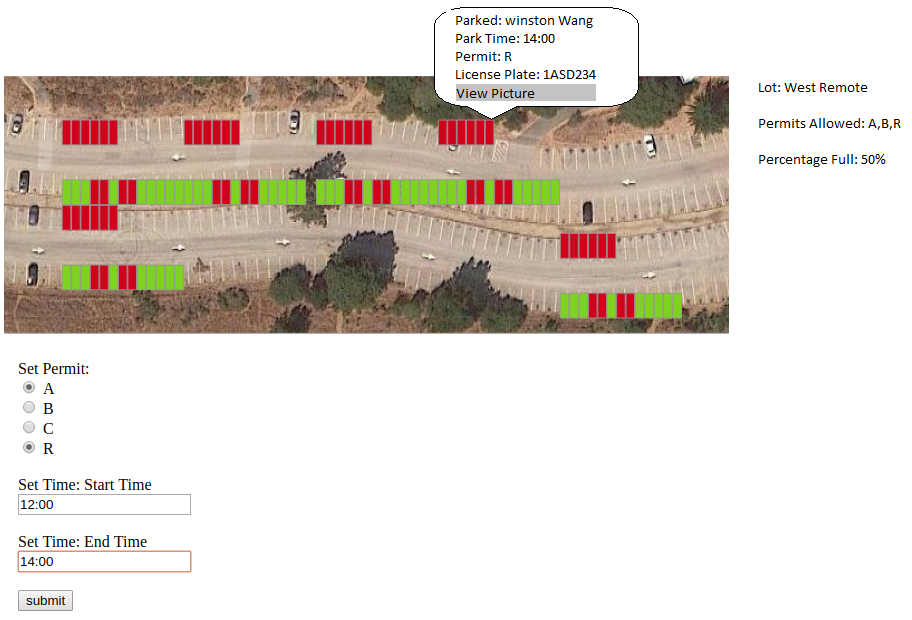
\includegraphics[width=15cm]{adminAppPics/lotPic.png}
\caption{screen of lot for administrator application}
\label{adminLotScreen}
\end{figure}

What we see here is a Google satellite image of the lot. Laid on top of the image are little green and red rectangles that represent the spots. Green is a free spot, red is an occupied spot. Then when the administrator clicks on a spot, a little bubble will appear with the spot's relevant information. Above we can see that the administrator has clicked on an occupied spot and so it shows that Winston Wang is parked there, He parked at 16:00, he possesses an R permit, and that his license plate is 1ASD234. And at the bottom of the little pop-up there is an option to see the picture that the sensor camera took to get the license plate. On the right of the image is a little blurb about the lot they are looking at. The lot is the West Remote parking lot, the permits currently allowed to park there are A,B,and R permit holders, and the lot is 50\% full.\\

Aside from observing the individual parking space, the administrator is also able to change the various parameters of the parking lot. On the preceding page, in figure 5.11 we see that the administrator is changing the permits that are allowed to park there and the times that they are able to park there. So, when the administrator hits the submit button the West Remote parking lot will only allow A and R permit holder to park there between the hours of 12:00 and 14:00. Then when it passes 14:00 it will continue on to default parking permits/times.\\

The administrator is also able to manipulate the individual parking spaces in certain ways. The administrator should be able to reserve parking spaces in case there is a guest visiting the school. If that happens and there is no parking, that would reflect very poorly on the school. So, when the administrator clicks on a free parking space, there is an additional prompt to set the parking spot to be reserved. When this happens the page will send a signal to the cloud to set that space to occupied. Then the mobile application will pull this information from the cloud and that particular parking space will be seen as reserved on the application, thus securing a spot for the school's important guest. This can be observed in the figure on the next page.\\

\begin{figure}[H]
\centering
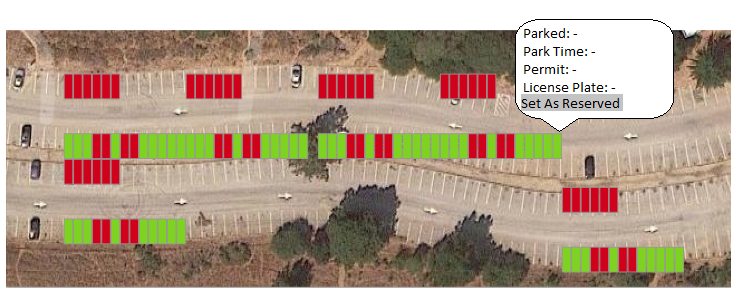
\includegraphics[width=15cm, height=5.5cm]{adminAppPics/lotPicReserve.png}
\caption{Administrator can reserve spots by clicking on unoccupied parking spots}
\label{adminReserve}
\end{figure}

Aside from looking at the individual parking spaces and the immediate fullness of the parking lot, the administrator should also be able to look at the general statistics of the parking lots. They should see charts and graphs that depict the usages of the parking lots on an average basis and be able to look at the usage charts. Figure \ref{adminStats} shows what this looks like.\\

\begin{figure}[!htb]
\centering
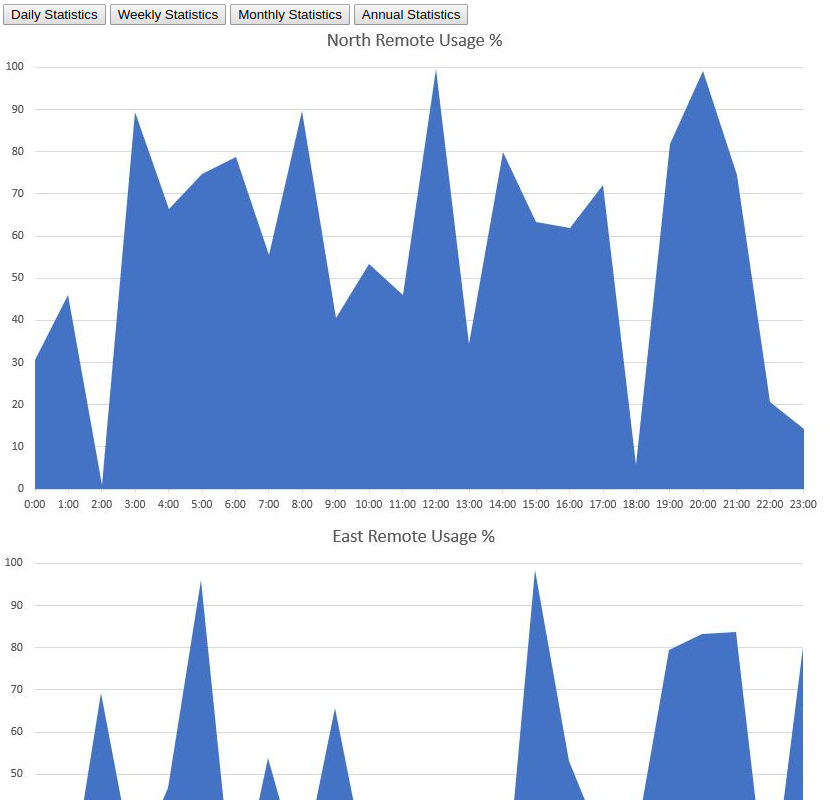
\includegraphics[width=13cm]{adminAppPics/statsPage.png}
\caption{Administrator can observe and analyze usage of the parking lots on multiple bases}
\label{adminStats}
\end{figure}

In Figure \ref{adminStats}, What we have above is fictitious data of the usage of the parking different parking lots throughout the day. As we can see in the figure, we can see how the North Remote parking lot becomes full and empty as the day progresses. At the top of the figure there are buttons that allow the administrator to look at the general usage of the parking lots over different time frames. They can observe weekly, monthly, and annual statistics of the usage of parking lots. Aside from those functionalities observed in the figure, we also have the ability to observe more focused statistics. For example, we have the ability to observe certain days of the week over certain time periods. This means we can observe the usage of the parking lot over all Tuesdays of a couple months. Then fro there the administrator and their team can use this information to update the system and help make the entire process of parking faster and more efficient.\\

\subsubsection{Administrative Application APIs}
The APIs of the administrative application are not so much APIs, but rather calls to APIs that are on the cloud. The cloud server will host written functions and scripts, and the administrative application will simply call the appropriate API based on what changes that the administrator will make. to see the APIs that the administrative application can call refer to section \ref{cloudAdminAPIs}\\

\section{Hardware Parts List}
The following list comprises of the hardware parts that were used to build and design the first prototype of the project.
\begin{table}[h]
\renewcommand{\arraystretch}{1.5}
%\caption{Parts list}
\centering
\begin{tabular}{|c|c|c|}
\hline
Quantity & Items & Price\\
\hline
2 & Raspberry Pi 3 & \$60\\
\hline
2 & Raspberry Zero & \$20\\
\hline
2 & Adapters for Pi Zero & \$30\\ %What kind of adapter is this?
\hline
2 & Arduino & \$10\\
\hline
2 & PAdafruit Pi Display & \$10\\
\hline
2 & LANDZO 7 Inch Touch Screen & \$86\\
\hline
2 & Pi Camera & \$26\\
\hline
2 & SR04 & \$10\\
\hline
\multicolumn{2}{|c|}{\textbf{Subtotal}} & \$252\\
\hline
\end{tabular}
\end{table}

\end{document}